% Chương 3: Đề xuất kiến trúc và khung quản trị niềm tin
\chapter{ĐỀ XUẤT KIẾN TRÚC VÀ KHUNG QUẢN TRỊ NIỀM TIN}

Chương này trình bày đóng góp lý thuyết trung tâm của nghiên cứu. Nội dung đi từ yêu cầu (Mục 3.1) qua nguyên tắc thiết kế (Mục 3.2) đến kiến trúc tổng thể (Mục 3.3), sau đó tập trung vào khung quản trị niềm tin (Mục 3.4) --- phần lấp đầy khoảng trống đã xác định ở Mục 2.8. Mục 3.5 đặc tả mô hình dữ liệu, Mục 3.6 đặc tả quy trình xác minh. Mục 3.7 phân tích mô hình đe dọa, qua đó kiểm tra lại tính đầy đủ của thiết kế. Hai mục cuối trình bày các đánh đổi và đối chiếu với các kiến trúc tham chiếu.

\section{Yêu cầu hệ thống}

\subsection{Mục tiêu thiết kế}

Hệ thống được thiết kế để giải quyết đồng thời hai bài toán mà Chương 2 đã chỉ ra là thuộc hai tầng khác nhau: xác minh kỹ thuật và quản trị thẩm quyền. Điều đó dẫn tới năm mục tiêu thiết kế, trong đó mục tiêu cuối là điểm phân biệt với các hệ thống định danh tự chủ thông thường.

Thứ nhất, hệ thống cung cấp một hạ tầng định danh phi tập trung cho mọi thực thể tham gia --- người học, cơ sở đào tạo, bên xác minh và cơ quan quản trị. Mỗi thực thể sở hữu một định danh độc lập với hệ thống thông tin của bất kỳ tổ chức nào, kiểm soát bằng khóa mật mã mà chủ thể giữ.

Thứ hai, hệ thống hỗ trợ toàn bộ vòng đời của chứng thực: cấp phát, lưu trữ trong ví của chủ thể, trình bày, xác minh và thu hồi. Việc xác minh phải thực hiện được mà không cần tương tác với đơn vị cấp phát.

Thứ ba, hệ thống bảo đảm khả năng liên thông giữa nhiều cơ sở: người học dùng cùng một định danh để tiếp nhận và quản lý chứng thực từ nhiều đơn vị trong hệ sinh thái, và trình bày chúng trong một lần xác minh duy nhất.

Thứ tư, hệ thống tuân theo nguyên tắc bảo vệ quyền riêng tư từ gốc \cite{Cavoukian2009}: dữ liệu cá nhân không được ghi lên hạ tầng công khai bất biến, chủ thể kiểm soát việc chia sẻ, và mọi thao tác quản trị đều để lại dấu vết kiểm chứng được.

Thứ năm, và quan trọng nhất đối với đóng góp của nghiên cứu, hệ thống xây dựng một khung quản trị niềm tin cho môi trường giáo dục liên trường, trong đó thẩm quyền cấp phát được thiết lập, giới hạn phạm vi, giới hạn thời hạn, ủy quyền lại và thu hồi theo cách mà bất kỳ bên thứ ba nào cũng kiểm chứng được công khai --- thay vì dựa vào uy tín hoặc vào một quy trình thủ công.

\subsection{Yêu cầu chức năng}

Các yêu cầu chức năng được xây dựng xoay quanh vòng đời chứng thực, đồng thời bổ sung nhóm yêu cầu về quản trị thẩm quyền mà mô hình ba bên thuần túy không bao gồm. Mỗi yêu cầu đi kèm một tiêu chí kiểm chứng có thể quan sát được; đây là điều kiện đã đặt ra ở Mục 1.5.1 khi chọn khung phương pháp khoa học thiết kế.

\begin{longtable}{|c|p{2.6cm}|p{4.4cm}|p{4.8cm}|p{1.3cm}|}
\caption{Danh sách yêu cầu chức năng\label{tab:functional-requirements}} \\
\hline
\textbf{Mã} & \textbf{Yêu cầu} & \textbf{Mô tả} & \textbf{Tiêu chí kiểm chứng} & \textbf{Kịch bản} \\
\hline
\endfirsthead

\hline
\textbf{Mã} & \textbf{Yêu cầu} & \textbf{Mô tả} & \textbf{Tiêu chí kiểm chứng} & \textbf{Kịch bản} \\
\hline
\endhead

\hline
\endfoot

\hline
\endlastfoot

F1 & Đăng ký định danh
& Mọi thực thể sinh khóa phía máy khách, dựng DID Document và đăng ký định danh kèm giá trị băm lên chuỗi
& Phân giải định danh thành công; giá trị băm tính lại khớp giá trị đã neo trên chuỗi
& KB1 \\ \hline

F2 & Xoay vòng khóa và giữ lịch sử phiên bản
& Chủ sở hữu cập nhật DID Document bằng chữ ký của khóa hiện tại; các phiên bản trước vẫn truy xuất được
& Cập nhật tăng số phiên bản; chứng thực cấp bằng khóa cũ vẫn xác minh được
& KB1 \\ \hline

F3 & Quản lý vòng đời thẩm quyền
& Cơ quan quản trị phê duyệt bên phát hành kèm phạm vi và thời hạn, cập nhật phạm vi, đình chỉ và thu hồi
& Phê duyệt thành công; thu hồi có hiệu lực ngay trong lần xác minh tiếp theo; mọi thao tác có mã giao dịch trên chuỗi
& KB2, KB5 \\ \hline

F4 & Ủy quyền nhiều cấp có ràng buộc
& Bên phát hành có bit ủy quyền phê duyệt được bên phát hành cấp dưới trong phạm vi hẹp hơn
& Phạm vi vượt tập cha bị từ chối; thời hạn vượt thời hạn cha bị từ chối; bit ủy quyền không truyền tiếp
& KB2 \\ \hline

F5 & Chuyển quyền gốc hai bước
& Quản trị viên gốc đề cử; người được đề cử tự ký để tiếp nhận; đề cử có thể bị hủy trước khi tiếp nhận
& Quyền chỉ chuyển sau khi người được đề cử ký; địa chỉ không được đề cử ký nhận sẽ thất bại
& KB2 \\ \hline

F6 & Cấp phát chứng thực
& Bên phát hành dựng chứng thực theo mô hình dữ liệu W3C, ký bằng khóa riêng và ghi bản ghi neo lên chuỗi
& Chứng thực hợp lệ về cấu trúc; chữ ký Ed25519 kiểm tra được; loại văn bằng ngoài phạm vi bị từ chối tại hợp đồng
& KB3 \\ \hline

F7 & Lưu trữ an toàn phía chủ thể
& Khóa riêng được mã hóa và chỉ lưu dạng bản mã trên thiết bị của chủ thể
& Bản mã AES-256-GCM \cite{NIST_SP800_38D}; không gói tin nào gửi lên dịch vụ chứa khóa riêng hoặc mật khẩu
& KB1 \\ \hline

F8 & Trình bày có chọn lọc
& Chủ thể dựng bản trình bày từ tập chứng thực mình chọn và ký bằng khóa riêng
& Bản trình bày chỉ chứa các chứng thực được chọn; chữ ký của chủ thể kiểm tra được
& KB4 \\ \hline

F9 & Xác minh tính toàn vẹn và quyền sở hữu
& Bên xác minh kiểm tra chữ ký của bên phát hành, chữ ký của chủ thể, và đối chiếu nội dung với giá trị băm đã neo
& Phát hiện được nội dung bị sửa sau khi cấp; phát hiện được bản trình bày do thực thể khác ký
& KB4, KB7 \\ \hline

F10 & Xác minh thẩm quyền độc lập
& Bên xác minh tra cứu trạng thái thẩm quyền của bên phát hành trực tiếp từ chuỗi
& Xác minh hoàn tất khi dịch vụ của bên phát hành không hoạt động; phát hiện bên phát hành đã bị thu hồi hoặc hết hạn ủy quyền
& KB4, KB5 \\ \hline

F11 & Quản lý trạng thái chứng thực
& Thu hồi, đình chỉ và kích hoạt lại chứng thực; trạng thái phản ánh ngay trong mọi lần xác minh sau đó
& Chứng thực bị thu hồi bị từ chối; chứng thực hợp lệ vẫn đạt; đơn vị hết hạn ủy quyền vẫn thu hồi được chứng thực mình đã cấp
& KB6, KB7 \\ \hline

F12 & Dấu vết kiểm toán
& Mọi thao tác thay đổi trạng thái đều được ghi nhận kèm chủ thể thực hiện, đối tượng và thời điểm
& Nhật ký trả về đúng các thao tác đã thực hiện với cùng bộ tên hành động ở mọi cài đặt của tầng dịch vụ
& KB2, KB6 \\ \hline

\end{longtable}


\subsection{Yêu cầu phi chức năng}

\begin{longtable}{|c|p{2.6cm}|p{4.6cm}|p{5.4cm}|}
\caption{Danh sách yêu cầu phi chức năng}
\label{tab:non-functional-requirements} \\

\hline
\textbf{Mã} & \textbf{Nhóm} & \textbf{Yêu cầu} & \textbf{Tiêu chí đo lường} \\
\hline
\endfirsthead

\hline
\textbf{Mã} & \textbf{Nhóm} & \textbf{Yêu cầu} & \textbf{Tiêu chí đo lường} \\
\hline
\endhead

\hline
\endfoot

\hline
\endlastfoot

N1 & Niềm tin &
Thẩm quyền của bên phát hành kiểm chứng được độc lập &
Tra cứu trạng thái thẩm quyền không cần liên hệ bên phát hành hay cơ quan quản trị, không cần tài khoản hay thỏa thuận trước \\ \hline

N2 & Niềm tin &
Mọi thay đổi quản trị để lại dấu vết bất biến &
Toàn bộ thao tác ghi sổ đăng ký tin cậy đều có mã giao dịch trên chuỗi; không có thao tác nào xóa hoặc sửa được lịch sử, kể cả từ quản trị viên gốc \\ \hline

N3 & Niềm tin &
Quy tắc phân quyền được thi hành ở nơi không thể bỏ qua &
Mọi quy tắc phân quyền nằm trong hợp đồng; gọi trực tiếp hợp đồng mà bỏ qua tầng dịch vụ vẫn bị chặn \\ \hline

N4 & An toàn &
Không có thông tin học thuật đọc trực tiếp được từ dữ liệu trên chuỗi &
Liệt kê đầy đủ các trường được ghi vào hợp đồng; không trường nào chứa nội dung văn bằng ở dạng đọc được. Lưu ý: tiêu chí này \textbf{không} đồng nghĩa với {``}không có dữ liệu cá nhân trên chuỗi{''} --- xem phân tích tại Mục 2.5.4 và Mục 3.5.1 \\ \hline

N5 & An toàn &
Khóa riêng không rời khỏi thiết bị của chủ thể &
Kiểm tra toàn bộ gói tin gửi lên dịch vụ, không gói tin nào chứa khóa riêng, mật khẩu hay cụm từ khôi phục \\ \hline

N6 & An toàn &
Phát hiện toàn bộ kịch bản gian lận được định nghĩa trước &
Mỗi kịch bản ở Mục 3.7.2 bị chặn, và thông điệp từ chối khớp đúng nguyên nhân thật chứ không do một phép kiểm khác chặn trước \\ \hline

N7 & Quyền riêng tư &
Chủ thể kiểm soát việc chia sẻ &
Bản trình bày chỉ chứa các chứng thực chủ thể chọn; không thành phần nào của hệ thống trình bày được chứng thực thay chủ thể \\ \hline

N8 & Phi tập trung &
Xác minh không phụ thuộc bên phát hành trực tuyến &
Xác minh hoàn tất khi dịch vụ của bên phát hành ngừng hoạt động, chỉ cần chuỗi và lớp lưu trữ ngoài chuỗi \\ \hline

N9 & Liên thông &
Tuân thủ chuẩn W3C DID Core và mô hình dữ liệu chứng thực &
Cấu trúc DID Document và chứng thực hợp lệ theo đặc tả \cite{W3C_DIDCore2022, W3C_VCDM2025}; các điểm chưa tuân thủ được liệt kê tường minh \\ \hline

N10 & Liên thông &
Tầng dịch vụ có hợp đồng giao diện ổn định, không phụ thuộc cài đặt &
Hai cài đặt độc lập trả cùng kết quả và cùng mã trạng thái cho cùng một yêu cầu, kể cả với dữ liệu vào không hợp lệ \\ \hline

N11 & Hiệu năng &
Thời gian xác minh ở mức chấp nhận được &
Phân vị 95 của các tuyến đọc không vượt 500\,ms dưới tải đồng thời. \textbf{Yêu cầu này không kiểm chứng được} trên cách thiết lập đo hiện tại --- xem phân tích tại Mục 4.9.6 \\ \hline

N12 & Hiệu năng &
Hệ thống không sinh lỗi chức năng dưới tải &
Không yêu cầu nào thất bại và không yêu cầu nào chạm hạn mức trong toàn bộ phép đo. Đây là một phép đếm nên không bị ảnh hưởng bởi nhiễu đo \\ \hline

N13 & Khả năng mở rộng &
Kiến trúc hỗ trợ mở rộng ngang &
Tầng dịch vụ không giữ trạng thái phiên; mọi trạng thái dùng chung nằm trong cơ sở dữ liệu dùng chung hoặc trên chuỗi \\ \hline

\end{longtable}


Một lưu ý về cách đặt yêu cầu phi chức năng. Các tiêu chí đo lường ở Bảng \ref{tab:non-functional-requirements} được phát biểu dưới dạng có thể làm cho thất bại, chứ không dưới dạng mô tả định tính. Chẳng hạn yêu cầu {``}dữ liệu cá nhân không được ghi lên chuỗi{''} được đo bằng việc liệt kê toàn bộ các trường được ghi vào hợp đồng và kiểm tra rằng không trường nào chứa dữ liệu cá nhân, thay vì bằng một khẳng định chung về nguyên tắc thiết kế. Cách phát biểu này xuất phát từ nhận định ở Mục 1.5.2: một tiêu chí không thể làm cho thất bại thì không chứng minh được điều gì.

\section{Nguyên tắc thiết kế}

Ba nguyên tắc sau được áp dụng xuyên suốt và được dùng làm căn cứ khi phải lựa chọn giữa các phương án.

\noindent \textbf{Nguyên tắc 1 --- Phi tập trung có kiểm soát.}

Hệ thống loại bỏ sự phụ thuộc vào một điểm xác minh trung tâm, nhưng không theo hướng phi tập trung tuyệt đối. Mô hình vẫn duy trì một nguồn niềm tin gốc đảm nhiệm việc quản trị thẩm quyền cấp phát. Điểm cần làm rõ là \emph{giới hạn} của quyền lực đó: nguồn niềm tin gốc quyết định ai được cấp phát loại văn bằng nào, nhưng không giữ dữ liệu của người học, không tham gia vào từng lần xác minh, và không có khả năng kỹ thuật để ký thay bất kỳ bên phát hành nào. Sự phân tách này là có chủ đích --- nó giữ lại đúng phần quyền lực mà thể chế thực sự cần, và loại bỏ phần quyền lực mà thể chế không cần nhưng lại tạo ra rủi ro tập trung.

\noindent \textbf{Nguyên tắc 2 --- Phân tách lớp với phụ thuộc một chiều.}

Hệ thống được phân thành bốn lớp, trong đó lớp trên phụ thuộc lớp dưới và không có chiều ngược lại. Hệ quả thực tiễn là mỗi lớp có thể thay thế độc lập: đổi phương thức DID ở lớp định danh không ảnh hưởng tới cấu trúc chứng thực ở lớp trên; mở rộng từ mô hình một nguồn niềm tin gốc sang mô hình liên hợp ở lớp quản trị không đòi hỏi thay đổi ba lớp dưới.

\noindent \textbf{Nguyên tắc 3 --- Mọi tuyên bố phải kiểm chứng được tại nguồn.}

Hệ thống không chấp nhận một tuyên bố chỉ vì nó đến từ một thành phần đáng tin cậy. Giá trị băm do phía máy khách khai báo đều được tính lại từ chính nội dung để đối chiếu; quyền hạn của một thực thể được kiểm trực tiếp trên chuỗi thay vì dựa vào vai trò ghi trong phiên đăng nhập; mọi bản ghi tham chiếu tới một giao dịch trên chuỗi đều được xác minh với nút đầy đủ trước khi ghi vào chỉ mục. Nguyên tắc này có một hệ quả quan trọng về cấu trúc dữ liệu: cơ sở dữ liệu quan hệ trong hệ thống chỉ là \emph{chỉ mục} phục vụ truy vấn nhanh, không phải nguồn sự thật. Nguồn sự thật là trạng thái trên chuỗi.

\section{Kiến trúc tổng thể}

\subsection{Các thực thể tham gia}

Hệ thống gồm bốn thực thể. Ba thực thể đầu là mô hình ba bên chuẩn của định danh tự chủ; thực thể thứ tư là điểm khác biệt so với một hệ thống thuần túy theo mô hình đó.

\begin{figure}[H]
    \centering
    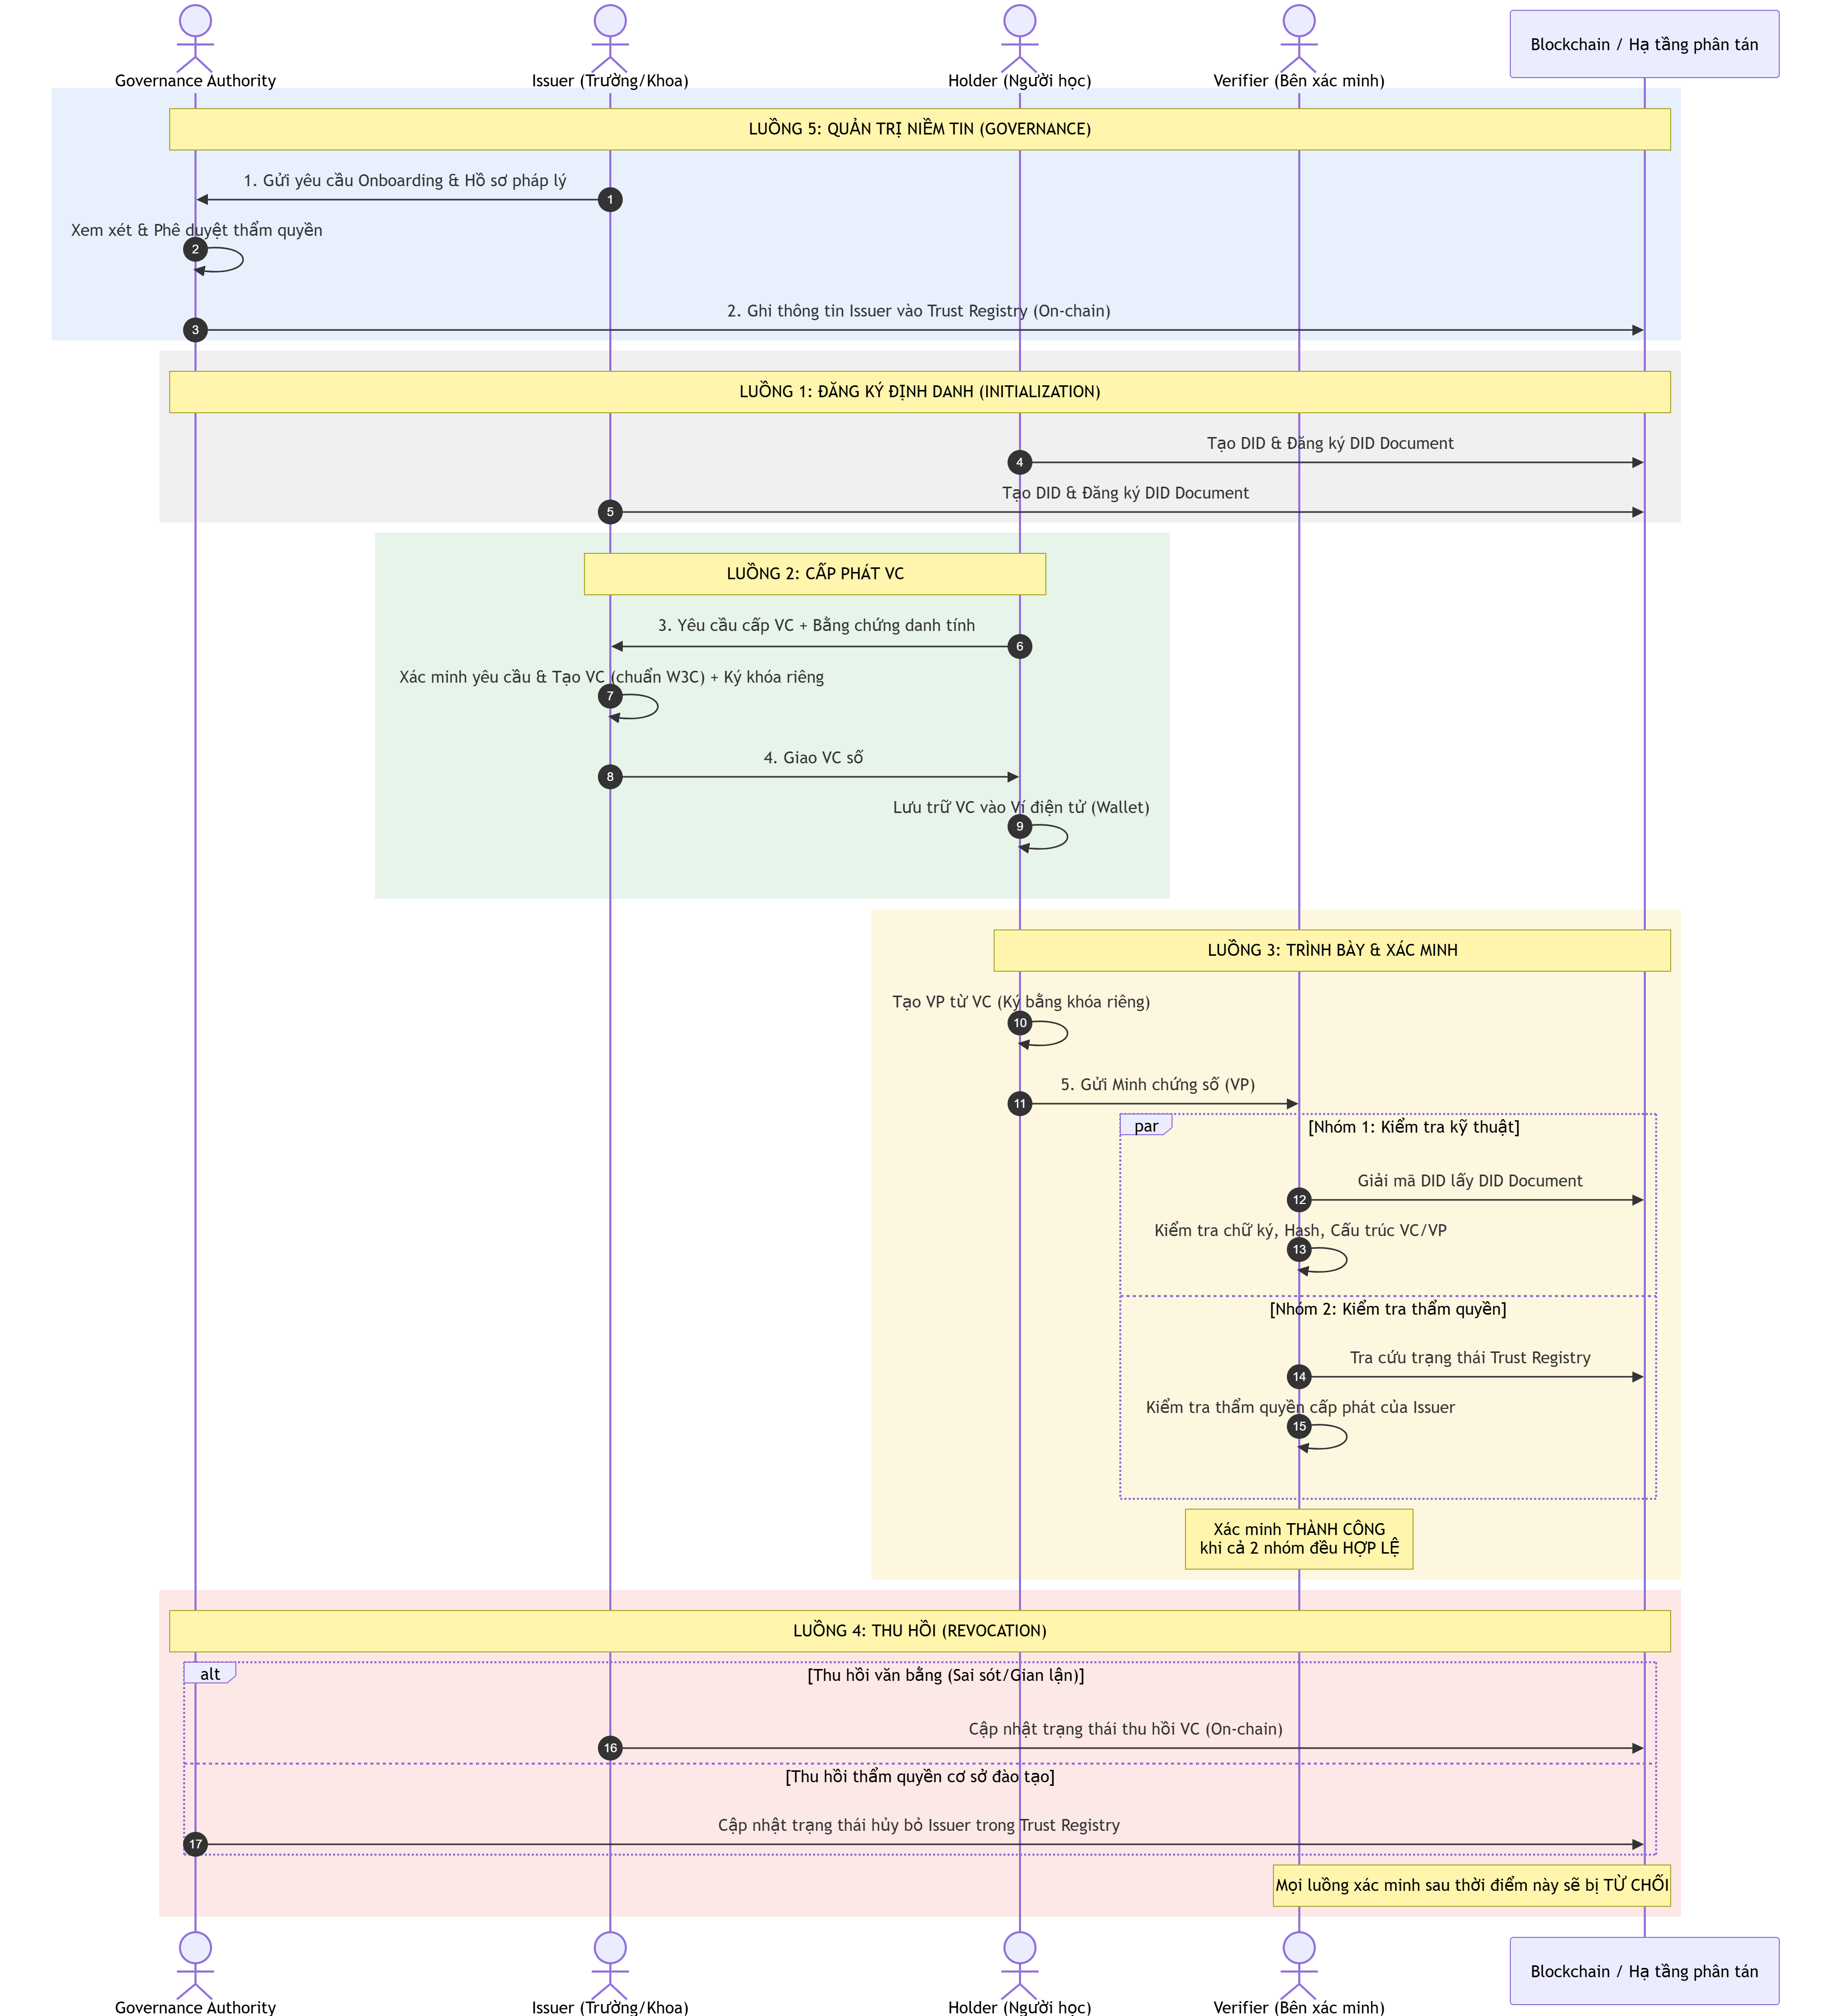
\includegraphics[width=0.75\textwidth]{images/system-flow.png}
    \caption{Luồng hoạt động tổng thể giữa bốn thực thể của hệ thống}
    \label{fig:system-workflow}
\end{figure}

\textbf{Cơ quan quản trị} (Governance Authority) là thực thể có thẩm quyền cao nhất trong hệ sinh thái. Trong bối cảnh ĐHQGHN, đây là cấp quản lý của ĐHQGHN hoặc đơn vị được ủy quyền về đảm bảo chất lượng. Cơ quan quản trị không tham gia vào luồng cấp phát hay xác minh thông thường; vai trò của nó là thiết lập và duy trì các quy tắc, cụ thể hóa qua việc quản lý sổ đăng ký tin cậy --- quyết định tổ chức nào được phép cấp phát, với phạm vi thẩm quyền nào, trong thời hạn nào, và thu hồi khi cần. Đây là nguồn niềm tin gốc của toàn hệ thống, nên khóa của nó cần mức bảo vệ cao nhất, và cơ chế chuyển quyền gốc là một điểm thiết kế quan trọng (Mục 3.4.4).

\textbf{Bên phát hành} (Issuer) là các đơn vị được cơ quan quản trị phê duyệt để cấp phát văn bằng --- các trường thành viên hoặc đơn vị đào tạo của ĐHQGHN. Mỗi bên phát hành có định danh riêng và bộ khóa riêng. Phạm vi thẩm quyền quy định những loại văn bằng mà đơn vị được phép cấp, và được ghi nhận trong sổ đăng ký tin cậy.

\textbf{Chủ thể} (Holder) là người học --- đối tượng của văn bằng, đồng thời là bên nhận và lưu giữ chứng thực trong ví định danh của mình. Chủ thể là thực thể duy nhất quyết định chia sẻ thông tin nào, với ai và khi nào.

\textbf{Bên xác minh} (Verifier) là bất kỳ bên nào cần kiểm chứng tính hợp lệ của văn bằng. Điểm quan trọng là bên xác minh không cần quan hệ đặc biệt nào với bên phát hành hay cơ quan quản trị; họ chỉ cần truy cập được hạ tầng công bố trạng thái.

\subsection{Luồng hoạt động}

Hệ thống vận hành qua năm luồng. Bốn luồng đầu tương ứng với vòng đời chứng thực; luồng thứ năm là luồng quản trị --- luồng diễn ra ít thường xuyên nhất nhưng có tác động dài hạn lớn nhất, và thường bị bỏ qua trong các mô tả về định danh tự chủ.

\noindent \textbf{Luồng 1 --- Đăng ký định danh.} Thực thể muốn tham gia hệ thống sinh cặp khóa, dựng DID Document chứa khóa công khai, ghim tài liệu đó lên lớp lưu trữ ngoài chuỗi để nhận một định danh nội dung, rồi ghi định danh cùng giá trị băm của tài liệu lên chuỗi. Sau bước này, bất kỳ ai cũng phân giải được DID để lấy khóa công khai và kiểm tra được tài liệu nhận về đúng là bản đã đăng ký.

\noindent \textbf{Luồng 2 --- Cấp phát chứng thực.} Chủ thể gửi yêu cầu cấp phát kèm bằng chứng về danh tính. Bên phát hành xác minh yêu cầu, dựng chứng thực theo chuẩn, ký bằng khóa riêng của mình, ghim nội dung lên lớp lưu trữ ngoài chuỗi, rồi ghi bản ghi neo lên chuỗi. Hợp đồng kiểm tra thẩm quyền của bên phát hành \emph{trước khi} ghi --- nghĩa là một đơn vị không có thẩm quyền sẽ thất bại ngay tại bước này, chứ không phải bị phát hiện về sau ở bước xác minh.

\noindent \textbf{Luồng 3 --- Trình bày và xác minh.} Chủ thể dựng bản trình bày từ các chứng thực mình chọn, ký bằng khóa riêng, và chuyển cho bên xác minh. Bên xác minh thực hiện một chuỗi kiểm tra gồm hai nhóm độc lập: nhóm kỹ thuật kiểm tra chữ ký và tính toàn vẹn; nhóm thẩm quyền tra cứu trạng thái của chứng thực và trạng thái của bên phát hành trên chuỗi. Chi tiết tại Mục 3.6.

\noindent \textbf{Luồng 4 --- Thu hồi chứng thực.} Khi cần thu hồi một chứng thực, bên có thẩm quyền cập nhật trạng thái trên chuỗi. Mọi lần xác minh sau đó phát hiện trạng thái này và từ chối chứng thực, dù chữ ký vẫn hợp lệ về mặt toán học.

\noindent \textbf{Luồng 5 --- Quản trị thẩm quyền.} Khi một tổ chức muốn trở thành bên phát hành, cơ quan quản trị xem xét và --- nếu phê duyệt --- ghi bản ghi thẩm quyền lên chuỗi kèm phạm vi và thời hạn. Thao tác này để lại dấu vết vĩnh viễn. Tương tự khi thu hồi: cơ quan quản trị cập nhật trạng thái, và từ thời điểm đó mọi chứng thực do đơn vị đó cấp sẽ không vượt qua bước kiểm tra thẩm quyền, dù chúng vẫn hợp lệ về mặt kỹ thuật. Điểm cần nhấn mạnh: cơ quan quản trị \emph{không} tự thực hiện thao tác này thông qua một dịch vụ trung gian --- chính người quản trị ký giao dịch từ ví của mình, và hợp đồng là bên quyết định thao tác đó có được phép hay không.

\subsection{Mô hình phân lớp}

Kiến trúc được tổ chức thành bốn lớp xếp chồng từ hạ tầng tới ứng dụng. Ba lớp đầu là các lớp kỹ thuật tương ứng với hạ tầng định danh tự chủ; lớp thứ tư là lớp quản trị.

\begin{figure}[H]
    \centering
    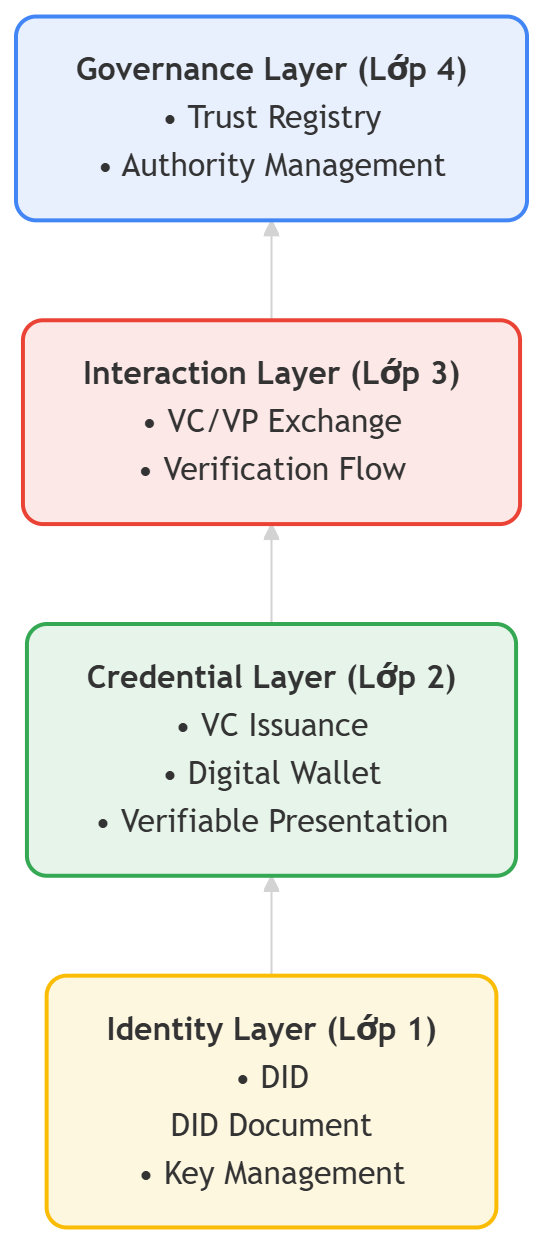
\includegraphics[width=0.3\textwidth]{images/layered_architecture.png}
    \caption{Mô hình kiến trúc phân lớp của hệ thống đề xuất}
    \label{fig:layered-architecture}
\end{figure}

\textbf{Lớp định danh} (Identity Layer) là nền của toàn hệ thống: cung cấp định danh duy nhất và bền vững cho mọi thực thể, cơ chế quản lý và xoay vòng khóa, và khả năng phân giải định danh thành thông tin kỹ thuật cần cho việc kiểm tra chữ ký.

\textbf{Lớp chứng thực} (Credential Layer) xây trên lớp định danh để thực hiện vòng đời văn bằng số: cấu trúc dữ liệu, cấp phát, lưu trữ, và quản lý trạng thái hiệu lực.

\textbf{Lớp tương tác} (Interaction Layer) định nghĩa cách các thực thể trao đổi: giao thức trình bày, quy trình xác minh, và cơ chế chia sẻ giữa các tổ chức.

\textbf{Lớp quản trị} (Governance Layer) lấp đầy khoảng trống về niềm tin thể chế và niềm tin quản trị: duy trì sổ đăng ký tin cậy, xử lý các quyết định phê duyệt và thu hồi, và cung cấp dữ liệu để lớp tương tác trả lời được câu hỏi {``}bên phát hành này có thẩm quyền hay không{''}.

Cần ghi nhận một điểm về cách trình bày. Như đã phân tích ở Mục 2.7.4, kiến trúc tham chiếu Trust over IP mô tả quản trị như một chiều xuyên suốt song song với chồng kỹ thuật, không phải một lớp riêng \cite{ToIP_GovMetamodel2022}. Cách nhìn đó chính xác hơn về mặt khái niệm, bởi các quyết định quản trị thực tế tác động tới cả bốn lớp. Nghiên cứu này vẫn trình bày quản trị thành một lớp riêng vì nó giúp mô tả rõ ranh giới trách nhiệm trong một hệ thống cụ thể, nhưng không xem đó là mô hình khái niệm đầy đủ.

\subsection{Các thành phần hệ thống}

\begin{longtable}{|p{2.8cm}|p{4.3cm}|p{2.1cm}|p{2.4cm}|p{2.4cm}|}
\caption{Các thành phần chính của hệ thống}
\label{tab:system-components} \\

\hline
\textbf{Thành phần} & \textbf{Trách nhiệm} & \textbf{Đầu vào chính} & \textbf{Đầu ra chính} & \textbf{Phụ thuộc} \\
\hline
\endfirsthead

\hline
\textbf{Thành phần} & \textbf{Trách nhiệm} & \textbf{Đầu vào chính} & \textbf{Đầu ra chính} & \textbf{Phụ thuộc} \\
\hline
\endhead

\hline
\endfoot

\hline
\endlastfoot

Sổ đăng ký định danh
& Đăng ký, cập nhật, thu hồi định danh; giữ lịch sử phiên bản DID Document
& Giá trị băm và định danh nội dung của DID Document
& Bản ghi định danh trên chuỗi
& Lớp lưu trữ ngoài chuỗi
\\ \hline

Sổ đăng ký tin cậy
& Lưu và công bố trạng thái thẩm quyền: phạm vi, thời hạn, trạng thái, phiên bản
& Địa chỉ của bên phát hành
& Bản ghi thẩm quyền trên chuỗi
& Sổ đăng ký định danh
\\ \hline

Sổ đăng ký chứng thực
& Neo giá trị băm của chứng thực và quản lý trạng thái hiệu lực
& Giá trị băm, định danh nội dung, loại và thời hạn
& Bản ghi chứng thực trên chuỗi
& Sổ đăng ký tin cậy, sổ đăng ký định danh
\\ \hline

Ví định danh số
& Sinh và bảo vệ khóa, ký chứng thực và ký giao dịch, dựng bản trình bày
& Mật khẩu hoặc cụm từ khôi phục
& Chữ ký, giao dịch đã ký, bản trình bày
& Không phụ thuộc tầng dịch vụ
\\ \hline

Tầng chuỗi phía máy khách
& Dựng giao dịch, lấy dạng tuần tự hóa từ nút đầy đủ, ký, gửi và chờ xác nhận
& Tên hàm và tham số
& Mã giao dịch đã xác nhận
& Ví định danh, nút đầy đủ
\\ \hline

Dịch vụ xác minh giao dịch
& Kiểm bốn điều kiện của giao dịch với nút đầy đủ trước khi ghi chỉ mục
& Mã giao dịch do máy khách khai báo
& Kết luận chấp nhận hoặc từ chối
& Nút đầy đủ
\\ \hline

Dịch vụ xác minh chứng thực
& Thực hiện bảy bước kiểm tra và trả báo cáo theo từng bước
& Bản trình bày
& Báo cáo xác minh chi tiết
& Toàn bộ sổ đăng ký, lớp lưu trữ ngoài chuỗi
\\ \hline

Tầng chỉ mục
& Lưu bản sao phục vụ truy vấn nhanh, nhật ký kiểm toán, dữ liệu danh sách
& Bản ghi đã được xác minh
& Kết quả truy vấn
& Cơ sở dữ liệu dùng chung
\\ \hline

Điểm vào dịch vụ
& Điều phối yêu cầu, xác thực phiên, giới hạn tần suất
& Yêu cầu HTTP
& Phản hồi theo hợp đồng giao diện
& Toàn bộ hệ thống
\\ \hline

\end{longtable}


Ba điểm về quan hệ giữa các thành phần cần được làm rõ.

Thứ nhất, \textbf{ví định danh là thành phần duy nhất vận hành hoàn toàn phía máy khách}. Toàn bộ thao tác sinh khóa, mã hóa và ký số được thực thi trong trình duyệt bằng Web Cryptography API \cite{W3C_WebCrypto} và các thư viện mật mã chạy phía máy khách; dữ liệu đã mã hóa được lưu cục bộ qua Indexed Database API \cite{W3C_IndexedDB}. Tầng dịch vụ không tham gia vào bất kỳ thao tác mật mã nào của chủ thể và không có khả năng kỹ thuật để ký thay chủ thể. Đây là điều kiện cần để tính tự chủ của chủ thể không chỉ là một tuyên bố về chính sách.

Thứ hai, \textbf{tầng chỉ mục không nằm trên đường tin cậy}. Dịch vụ chỉ mục tồn tại để trả lời nhanh các truy vấn danh sách và lịch sử; nếu nó trả về dữ liệu sai, kết quả xác minh vẫn không bị ảnh hưởng, bởi mọi kết luận về tính hợp lệ đều được kiểm lại với chuỗi và với nội dung thực. Tính chất này là hệ quả trực tiếp của Nguyên tắc 3.

Thứ ba, \textbf{các thao tác ghi trạng thái lên chuỗi đều do chính chủ thể ký}. Dịch vụ không giữ khóa của bất kỳ vai trò nào, nên nó không thể khởi tạo một thao tác thay đổi trạng thái. Vai trò của nó trong các luồng ghi là xác minh rằng giao dịch mà máy khách khai báo thực sự tồn tại và đúng như khai báo, trước khi cập nhật chỉ mục.

\begin{figure}[H]
    \centering
    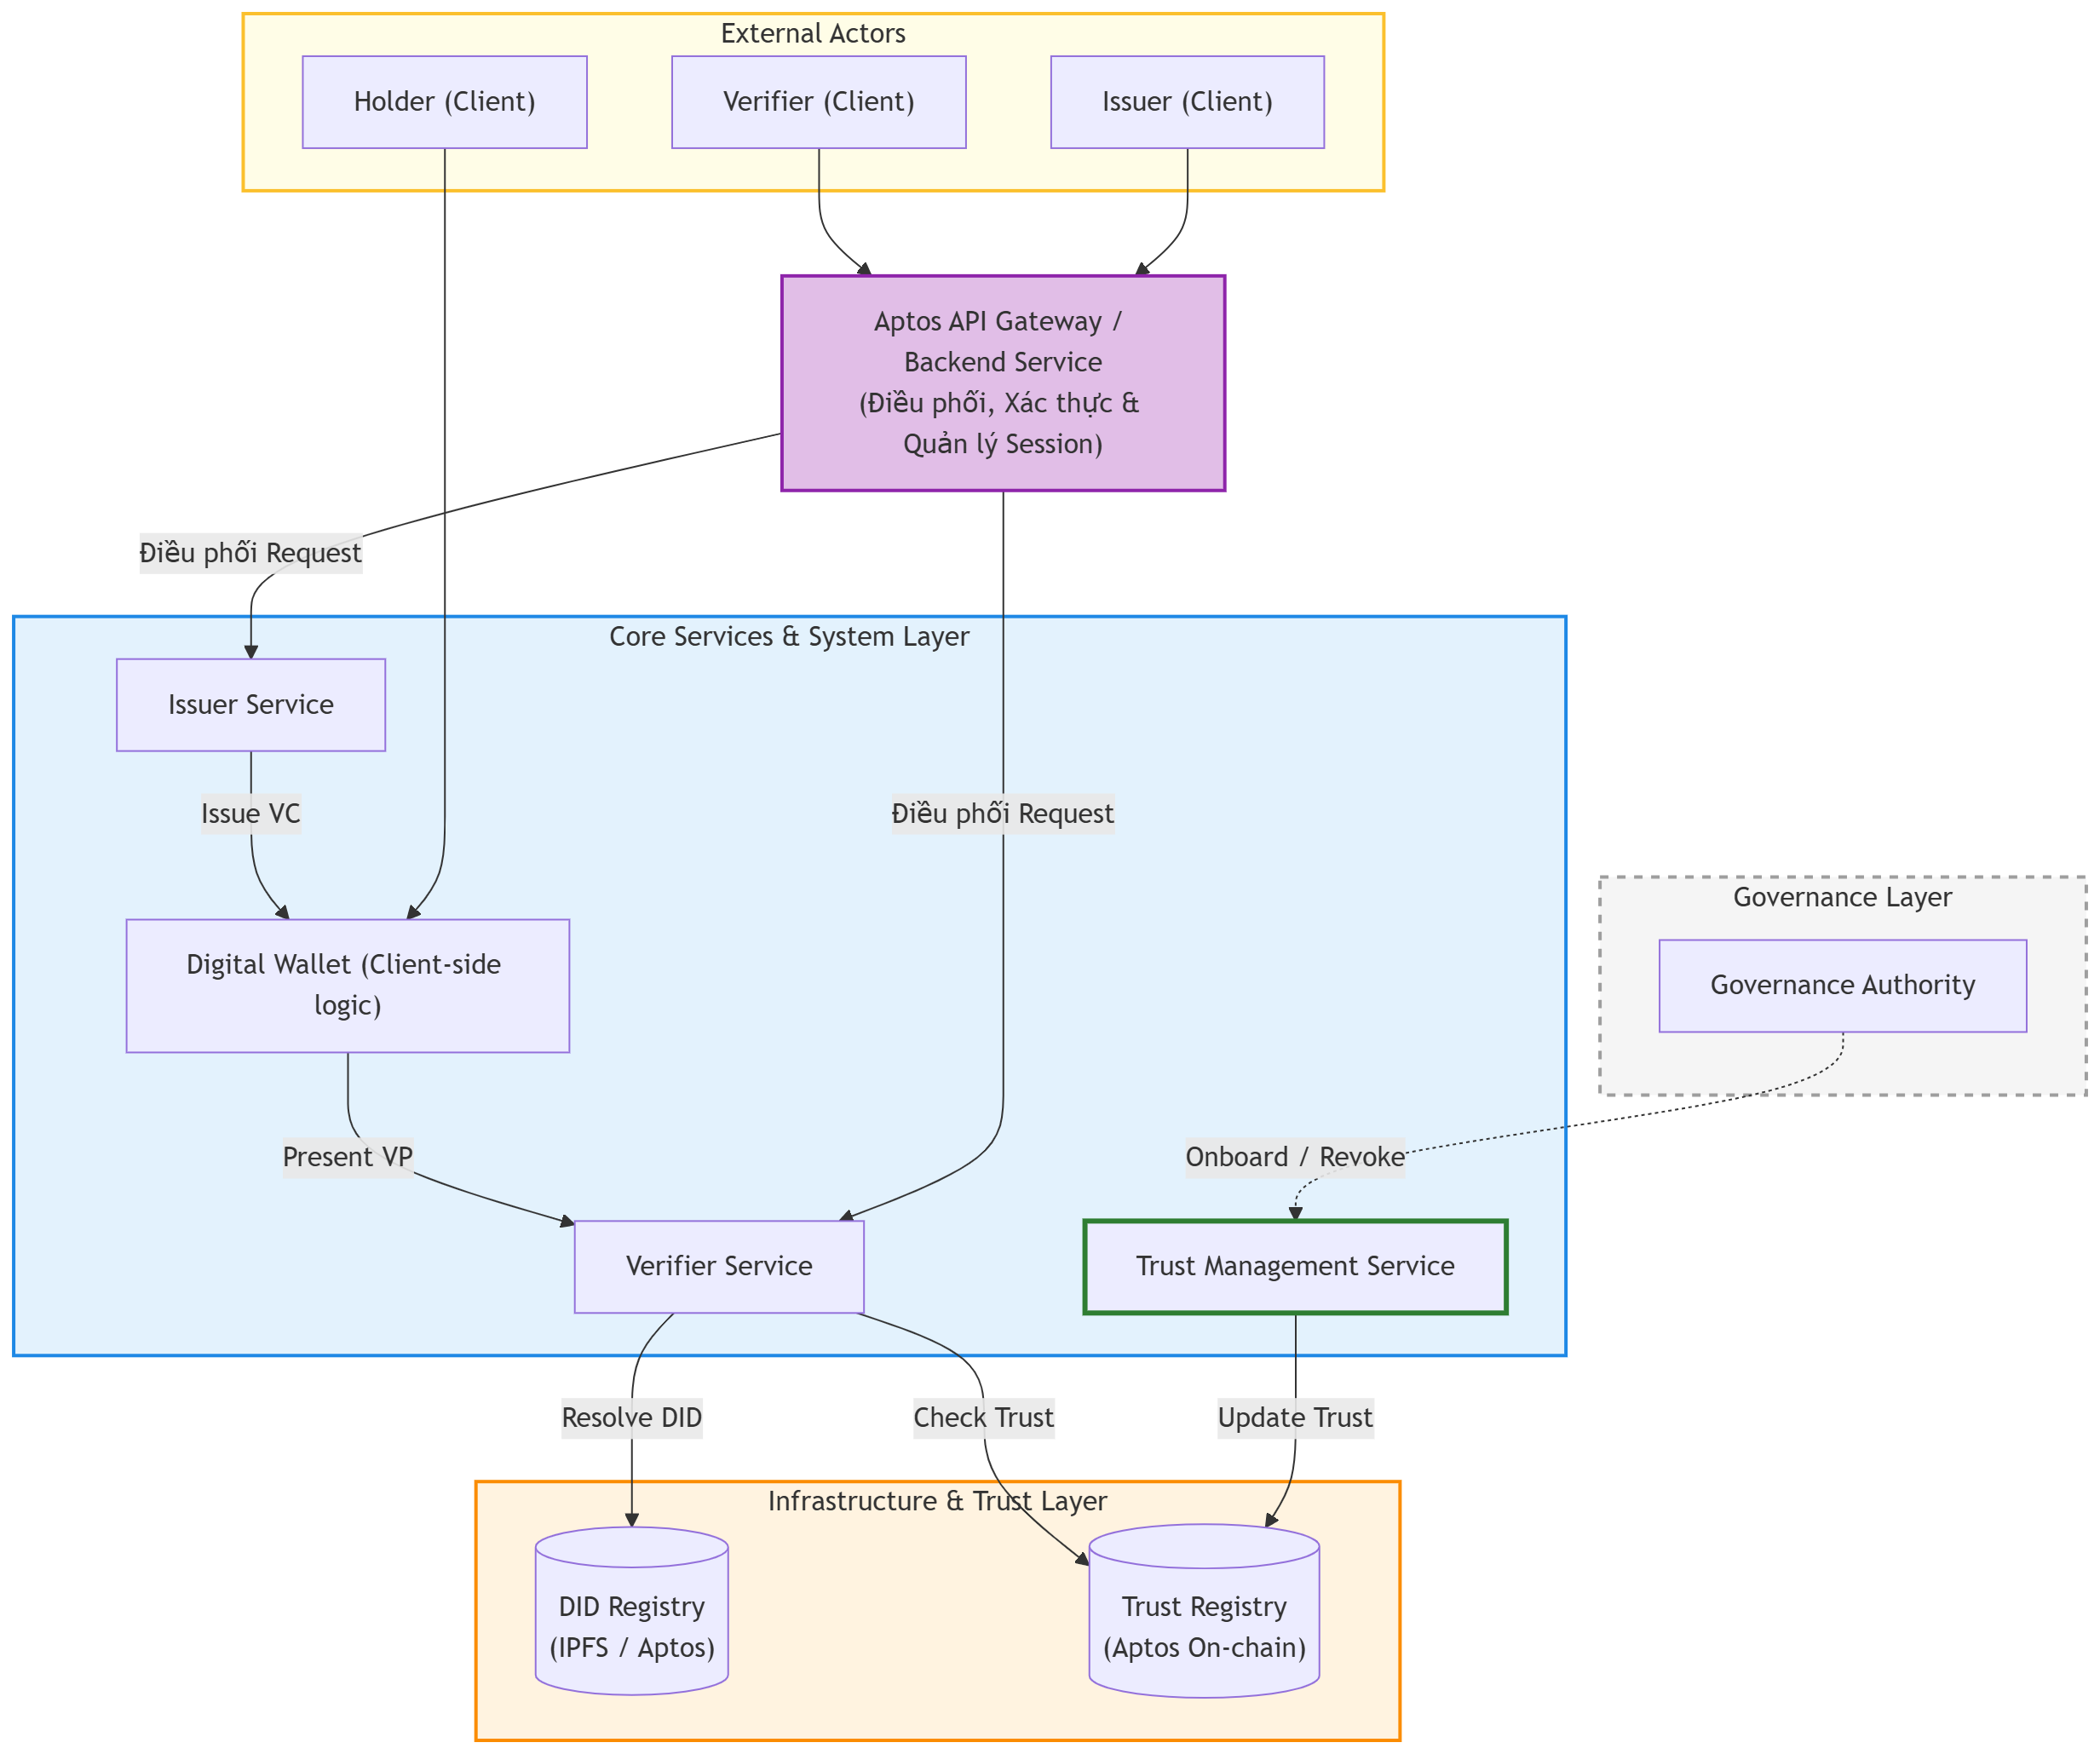
\includegraphics[width=1\textwidth]{images/system-architecture-components.png}
    \caption{Quan hệ giữa các thành phần của hệ thống}
    \label{fig:system-architecture-components}
\end{figure}

\section{Khung quản trị niềm tin}

\subsection{Vấn đề khởi tạo niềm tin}

Trước khi mô tả khung quản trị, cần xử lý một câu hỏi nền tảng mà mọi hệ thống niềm tin đều phải đối mặt: nếu mọi niềm tin đều cần được một cấp trên xác nhận, thì cấp cao nhất lấy niềm tin từ đâu?

Câu trả lời là: không lấy từ bên trong hệ thống kỹ thuật. Nguồn niềm tin gốc không thể tự chứng minh thẩm quyền của mình bằng cơ chế mật mã, bởi mọi bằng chứng mà nó tạo ra đều chỉ chứng minh rằng nó giữ một khóa cụ thể --- điều mà bất kỳ ai cũng làm được. Thẩm quyền của nguồn niềm tin gốc đến từ sự công nhận bên ngoài hệ thống: pháp lý, thể chế và xã hội. Trong trường hợp này, ĐHQGHN là nguồn niềm tin gốc không phải vì hệ thống kỹ thuật chứng minh được điều đó, mà vì ĐHQGHN được công nhận theo Luật Giáo dục đại học và có tư cách pháp nhân rõ ràng.

Nhận thức này không phải sự thừa nhận một thất bại mà là một định hướng thiết kế. Hệ thống kỹ thuật không cố thay thế sự công nhận thể chế; nó làm cho sự công nhận đó trở nên kiểm chứng được. Nói cách khác, hệ thống chuyển câu hỏi từ

\begin{quote}
{``}ĐHQGHN có đáng tin cậy hay không?{''} --- một câu hỏi thuộc phạm trù thể chế,
\end{quote}

thành

\begin{quote}
{``}Đơn vị này có đang được ĐHQGHN ủy quyền cấp loại văn bằng này hay không, và tôi có thể kiểm chứng điều đó mà không cần hỏi bất kỳ ai?{''} --- một câu hỏi trả lời được hoàn toàn bằng kỹ thuật.
\end{quote}

Đây là sự chuyển đổi mà cả tài liệu kỹ thuật của EBSI cũng nêu rõ dưới dạng nguyên tắc: sổ cái ghi nhận các quyết định về niềm tin nhưng không tạo ra chúng \cite{EBSI_TrustModel}.

\subsection{Chuỗi thẩm quyền và phạm vi cấp phát}

Khung quản trị biểu diễn thẩm quyền thành một chuỗi phân cấp có bốn mức, phản ánh đúng cấu trúc thể chế mô tả ở Mục 2.6.2.

\begin{figure}[H]
    \centering
    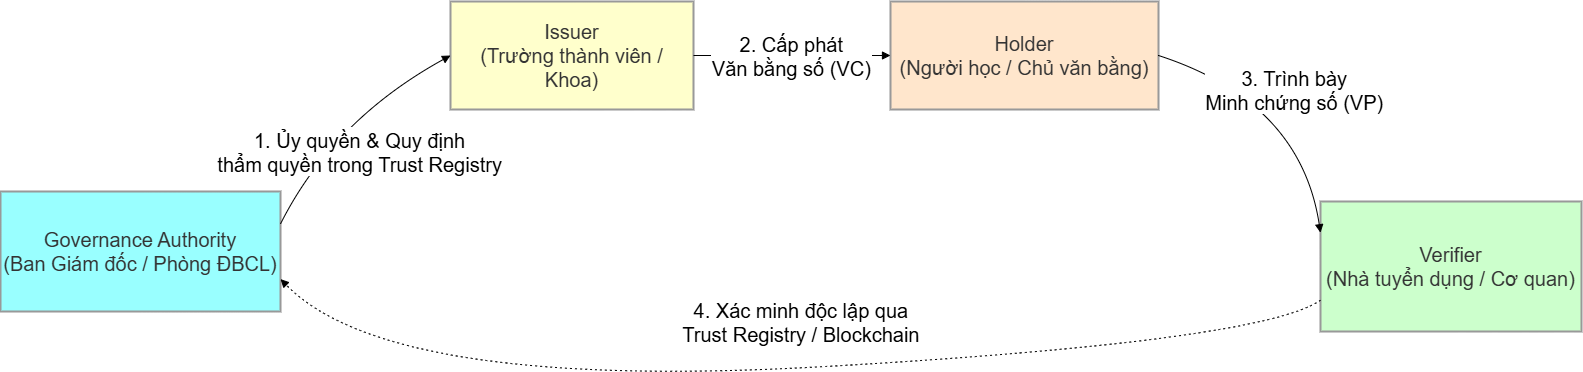
\includegraphics[width=1\textwidth]{images/system-interaction.png}
    \caption{Chuỗi niềm tin và các quan hệ ủy quyền trong hệ thống}
    \label{fig:system-interaction}
\end{figure}

Ở gốc là \textbf{quản trị viên gốc} (root), thực thể duy nhất và được xác lập tại thời điểm khởi tạo hệ thống. Quản trị viên gốc cấp quyền cho các \textbf{quản trị viên} (admin), là các đơn vị được giao nhiệm vụ quản lý việc phê duyệt bên phát hành. Quản trị viên phê duyệt các \textbf{bên phát hành} (issuer) kèm phạm vi thẩm quyền. Bên phát hành có bit ủy quyền đặc biệt có thể phê duyệt \textbf{bên phát hành cấp dưới} (sub-issuer) trong phạm vi hẹp hơn của mình (Mục 3.4.3).

Điểm thiết kế quan trọng là \textbf{cách biểu diễn phạm vi thẩm quyền}. Như đã nêu ở Mục 2.8, phần lớn hệ thống hiện có chỉ biểu diễn thẩm quyền ở dạng nhị phân. Thiết kế này dùng một mặt nạ bit để biểu diễn tập các loại văn bằng mà một đơn vị được phép cấp: mỗi loại ứng với một bit, và phạm vi thẩm quyền của đơn vị là phép hợp của các bit tương ứng.

\begin{table}[H]
\centering
\caption{Biểu diễn phạm vi thẩm quyền bằng mặt nạ bit}
\label{tab:vc-type-mask}
\renewcommand{\arraystretch}{1.25}
\begin{tabular}{|c|c|p{4.6cm}|p{5.2cm}|}
\hline
\textbf{Bit} & \textbf{Giá trị} & \textbf{Loại chứng thực} & \textbf{Ghi chú} \\
\hline
0 & 1  & Bằng cử nhân / kỹ sư & \\ \hline
1 & 2  & Bằng thạc sĩ & \\ \hline
2 & 4  & Bằng tiến sĩ & \\ \hline
3 & 8  & Bảng điểm, kết quả học tập & \\ \hline
4 & 16 & Chứng nhận vi mô, chứng chỉ ngắn hạn & \\ \hline
5 & 32 & Chứng thực ủy quyền & Chỉ quản trị viên gốc được cấp bit này; cho phép đơn vị phê duyệt bên phát hành cấp dưới \\ \hline
\end{tabular}
\end{table}

\noindent Phạm vi thẩm quyền của một đơn vị là phép hợp các giá trị tương ứng. Ví dụ, một trường được phép cấp bằng cử nhân, bằng thạc sĩ và bảng điểm có phạm vi $M = 1 \vee 2 \vee 8 = 11$. Phép kiểm tra {``}đơn vị này có được cấp loại $T$ hay không{''} rút về điều kiện $M \wedge T \neq 0$, còn phép kiểm tra {``}phạm vi $A$ là tập con của phạm vi $B$ hay không{''} rút về điều kiện $A \wedge \neg B = 0$. Cả hai đều có chi phí không đổi, không phụ thuộc số loại văn bằng trong phạm vi.


Cách biểu diễn này có ba ưu điểm thực tiễn. Thao tác kiểm tra {``}đơn vị này có được phép cấp loại văn bằng $T$ hay không{''} trở thành một phép giao bit duy nhất, nên chi phí không đổi dù phạm vi rộng hay hẹp. Thao tác kiểm tra {``}phạm vi $A$ có là tập con của phạm vi $B$ hay không{''} --- cần thiết cho việc ủy quyền lại --- cũng rút về một phép bit. Và toàn bộ phạm vi thẩm quyền được lưu trong một số nguyên duy nhất, nên không làm tăng đáng kể chi phí lưu trữ trên chuỗi. Giới hạn là số loại văn bằng tối đa bằng độ rộng của số nguyên được chọn; với một số nguyên 64 bit, giới hạn này đủ rộng cho bài toán hiện tại và có thể mở rộng bằng cách dùng nhiều từ hoặc chuyển sang sổ đăng ký loại dựa trên chuỗi định danh.

Ngoài phạm vi, mỗi bản ghi thẩm quyền còn mang \textbf{thời hạn ủy quyền}. Trường này cho phép biểu diễn đúng thực tiễn quản trị: một đơn vị được phép cấp bằng trong một chu kỳ kiểm định, và thẩm quyền tự hết hiệu lực khi chu kỳ kết thúc nếu không được gia hạn. Giá trị không được đặt tương ứng với ủy quyền vô thời hạn, hợp lý với một số loại thẩm quyền nhưng không nên là mặc định.

\subsection{Ủy quyền nhiều cấp}

Một yêu cầu thực tiễn mà các hệ thống hiện có chưa xử lý --- và như đã nêu ở Mục 2.6.3, chính đặc tả chuẩn hóa còn hoãn sang phiên bản sau --- là ủy quyền nhiều cấp: một trường thành viên được ĐHQGHN ủy quyền có thể cần ủy quyền tiếp cho một khoa hoặc một đơn vị trực thuộc.

Nếu cho phép ủy quyền lại không giới hạn, chuỗi thẩm quyền sẽ mất ý nghĩa: một đơn vị được phép cấp bằng cử nhân có thể ủy quyền cho đơn vị khác quyền cấp bằng tiến sĩ, hoặc ủy quyền với thời hạn dài hơn thời hạn của chính mình. Vì vậy thiết kế đặt ba ràng buộc, và cả ba được thi hành bởi hợp đồng chứ không bởi quy trình hành chính:

\begin{itemize}
    \item \textbf{Phạm vi phải là tập con.} Phạm vi mà bên ủy quyền trao cho cấp dưới phải là tập con của phạm vi mà chính họ đang có. Không thể trao thứ mình không có.
    \item \textbf{Thời hạn không được vượt quá thời hạn của bên ủy quyền.} Một ủy quyền phái sinh không thể sống lâu hơn ủy quyền gốc của nó.
    \item \textbf{Bit ủy quyền không được truyền tiếp.} Bên phát hành cấp dưới không nhận được quyền ủy quyền lại. Ràng buộc này giới hạn độ sâu của chuỗi ở hai cấp, và đó là lựa chọn có chủ đích: một chuỗi ủy quyền sâu không giới hạn khiến việc truy vết trách nhiệm trở nên bất khả thi trong thực tế, trong khi lợi ích thu được không rõ ràng. Riêng bit ủy quyền chỉ quản trị viên gốc được cấp.
\end{itemize}

Mỗi quan hệ ủy quyền còn được gắn với một \emph{chứng thực ủy quyền} --- một chứng thực do bên ủy quyền ký, xác nhận phạm vi được trao. Nội dung chứng thực được lưu ngoài chuỗi và giá trị băm cùng định danh nội dung của nó được ghi vào bản ghi thẩm quyền. Nhờ đó bên xác minh có thể truy xuất và kiểm tra bằng chứng về quan hệ ủy quyền, chứ không chỉ đọc một cờ trạng thái. Để tránh biến yêu cầu này thành gánh nặng vô ích, hợp đồng chỉ bắt buộc có chứng thực ủy quyền khi thực sự có quan hệ ủy quyền --- tức khi đơn vị được cấp bit ủy quyền, hoặc khi chính nó được phê duyệt bởi một bên phát hành chứ không phải bởi quản trị viên.

\subsection{Chuyển quyền gốc gồm hai bước}

Quản trị viên gốc là điểm tập trung quyền lực duy nhất của hệ thống, nên cơ chế chuyển quyền gốc là một điểm thiết kế có hệ quả đặc biệt lớn. Thiết kế trực quan nhất --- một thao tác duy nhất trong đó quản trị viên gốc hiện tại chỉ định địa chỉ của người kế nhiệm --- có một khuyết điểm nghiêm trọng mà chỉ bộc lộ khi đã quá muộn: nó không có cơ chế nào kiểm tra rằng địa chỉ đích thực sự có người kiểm soát.

Nếu địa chỉ đích bị gõ sai, hoặc thuộc về một khóa đã mất, quyền quản trị gốc chuyển tới một địa chỉ không ai điều khiển được. Hệ thống không hỏng ngay --- các thao tác cấp phát và xác minh vẫn chạy bình thường --- nhưng toàn bộ năng lực quản trị bị mất vĩnh viễn: không thể phê duyệt bên phát hành mới, không thể thu hồi bên phát hành cũ, và không thể sửa chính sai sót đó. Vì trạng thái trên chuỗi là bất biến, không có cách khắc phục nào ngoài việc triển khai lại toàn bộ hệ thống ở một địa chỉ mới.

Thiết kế vì vậy tách thao tác này thành hai bước:

\begin{enumerate}
    \item \textbf{Đề cử.} Quản trị viên gốc hiện tại ghi địa chỉ của người được đề cử vào trạng thái chờ. Quyền quản trị \emph{chưa} chuyển.
    \item \textbf{Ký nhận.} Người được đề cử tự ký một giao dịch để tiếp nhận. Chỉ khi giao dịch này thành công thì quyền mới chuyển.
\end{enumerate}

Cùng với đó là thao tác thứ ba --- \textbf{hủy đề cử} --- cho phép quản trị viên gốc rút lại đề cử trước khi nó được tiếp nhận.

Giá trị của thiết kế này nằm ở bước thứ hai, và chính xác hơn là ở \emph{bản chất của chữ ký} trong bước đó. Chữ ký của người được đề cử là bằng chứng mật mã duy nhất cho thấy họ thực sự kiểm soát khóa riêng tương ứng với địa chỉ đã nêu --- điều mà một thao tác một bước không bao giờ chứng minh được. Đây là một trường hợp cụ thể của một nguyên tắc tổng quát hơn: khi một thao tác không thể hoàn tác, điều kiện tiên quyết của nó phải được chứng minh bằng hành động của bên bị ảnh hưởng, không phải bằng khai báo của bên thực hiện.

\subsection{Nguyên tắc bất đối xứng giữa cấp và thu hồi}

Nguyên tắc thiết kế thứ hai được rút ra trong quá trình xây dựng hệ thống liên quan tới quan hệ giữa thao tác cấp và thao tác thu hồi.

Cách thiết kế tự nhiên là đối xứng: nếu một đơn vị cần thẩm quyền còn hiệu lực để cấp văn bằng, thì nó cũng cần thẩm quyền còn hiệu lực để thu hồi văn bằng. Logic nghe hợp lý nhưng dẫn tới một kết quả sai trong tình huống quan trọng nhất.

Xét kịch bản sau. Một trường thành viên có thẩm quyền cấp bằng đến hết năm 2026. Năm 2027, trường phát hiện một văn bằng mình đã cấp năm 2025 là kết quả của gian lận. Với thiết kế đối xứng, trường không thu hồi được văn bằng đó, vì thẩm quyền của họ đã hết hạn. Văn bằng gian lận tiếp tục vượt qua mọi phép xác minh. Tình huống tương tự xảy ra khi thẩm quyền của một đơn vị bị thu hồi vì phát hiện sai phạm --- đúng lúc cần thu hồi các văn bằng đã cấp nhất thì năng lực thu hồi lại bị khóa.

Phân tích này dẫn tới nguyên tắc: \textbf{thao tác thu hồi luôn phải dễ hơn thao tác cấp}. Cụ thể, trong thiết kế:

\begin{itemize}
    \item Cấp phát chứng thực đòi hỏi thẩm quyền \emph{còn hiệu lực} và loại văn bằng nằm \emph{trong phạm vi} được phép.
    \item Thu hồi chứng thực chỉ đòi hỏi \emph{quyền sở hữu} --- bên thu hồi đúng là bên đã cấp chứng thực đó --- và định danh của bên đó còn hoạt động. Không kiểm tra thẩm quyền còn hiệu lực, không kiểm tra phạm vi.
    \item Một chứng thực đã hết hạn vẫn thu hồi được. Điều này thoạt nghe vô nghĩa, nhưng thu hồi và hết hạn mang hai thông điệp khác nhau: hết hạn nói rằng chứng thực không còn giá trị \emph{từ thời điểm nào đó}; thu hồi nói rằng chứng thực \emph{chưa bao giờ} đáng tin. Thông điệp thứ hai cần được phát ra kể cả khi chứng thực đã hết hạn, vì nó là một tuyên bố vĩnh viễn về gian lận.
\end{itemize}

Nguyên tắc này có một phát biểu tổng quát: trong hệ thống an toàn, các thao tác làm giảm quyền hoặc giảm độ tin cậy nên có điều kiện tiên quyết lỏng hơn các thao tác làm tăng chúng. Điều kiện chặt ở thao tác giảm không bảo vệ hệ thống mà chỉ ngăn hệ thống tự sửa lỗi.

\subsection{Dấu vết kiểm toán và khôi phục vai trò}

Hai yêu cầu đối lập cần được xử lý cùng nhau: mọi thay đổi quản trị phải để lại dấu vết không thể xóa, và một đơn vị bị thu hồi thẩm quyền phải có thể được cấp lại sau khi khắc phục sai phạm.

Nếu bản ghi thẩm quyền bị ghi đè khi cấp lại, dấu vết kiểm toán sẽ mất. Nếu không cho cấp lại, hệ thống không phản ánh được thực tiễn --- một đơn vị bị đình chỉ rồi được phục hồi sau kiểm định là tình huống bình thường. Thiết kế giải quyết bằng cách tách hai thứ: bảng tra cứu {``}đơn vị $A$ hiện ứng với bản ghi nào{''} được cập nhật, còn bản ghi cũ vẫn nằm nguyên trong tập các bản ghi. Mỗi bản ghi mang một số \textbf{phiên bản} tăng dần theo mỗi lần được cấp lại. Nhờ đó lịch sử đầy đủ của một đơn vị --- được cấp quyền lần nào, bị thu hồi khi nào vì lý do gì, được phục hồi khi nào --- đều truy xuất được, trong khi truy vấn trạng thái hiện tại vẫn là một phép tra cứu trực tiếp.

Cơ chế tương tự áp dụng cho định danh. Khi khóa riêng của một thực thể bị lộ, hành động đúng là thu hồi định danh cũ và đăng ký định danh mới bằng khóa mới. Nếu hệ thống khóa một địa chỉ vào đúng một định danh vĩnh viễn, thì sự cố lộ khóa đồng nghĩa với mất địa chỉ vĩnh viễn. Thiết kế cho phép đăng ký định danh mới sau khi định danh cũ đã bị thu hồi, đồng thời giữ định danh cũ trong sổ với trạng thái đã thu hồi --- để các chứng thực được cấp bằng khóa cũ vẫn tra cứu được và vẫn phản ánh đúng trạng thái.

\subsection{Phân tách thẩm quyền theo thao tác}

Một nội dung của khung quản trị là việc quy định thao tác nào thuộc vai trò nào. Các quy định này không phải lựa chọn tùy ý mà xuất phát từ yêu cầu phân tách trách nhiệm.

\begin{longtable}{|p{4.3cm}|p{3.2cm}|p{6.5cm}|}
\caption{Phân tách thẩm quyền theo thao tác}
\label{tab:role-permission} \\

\hline
\textbf{Thao tác} & \textbf{Vai trò được phép} & \textbf{Cơ sở của quy định} \\
\hline
\endfirsthead

\hline
\textbf{Thao tác} & \textbf{Vai trò được phép} & \textbf{Cơ sở của quy định} \\
\hline
\endhead

\hline
\endfoot

\hline
\endlastfoot

Cấp và thu hồi quyền quản trị viên
& Chỉ quản trị viên gốc
& Quyền phê duyệt bên phát hành là quyền có hệ quả rộng nhất, nên việc trao quyền đó phải tập trung ở gốc
\\ \hline

Cấp bit ủy quyền cho bên phát hành
& Chỉ quản trị viên gốc
& Bit này cho phép mở rộng chuỗi thẩm quyền; nếu quản trị viên cấp được thì chuỗi có thể mở rộng ngoài kiểm soát của gốc
\\ \hline

Phê duyệt bên phát hành (không kèm bit ủy quyền)
& Quản trị viên gốc, quản trị viên
& Đây là thao tác quản trị thường xuyên, cần phân cấp để vận hành được
\\ \hline

Phê duyệt bên phát hành cấp dưới
& Bên phát hành có bit ủy quyền
& Phạm vi phải là tập con, thời hạn không vượt thời hạn của bên ủy quyền, bit ủy quyền không truyền tiếp
\\ \hline

Đình chỉ, kích hoạt lại, thu hồi bên phát hành
& Quản trị viên gốc, quản trị viên
& Thao tác làm giảm quyền, nên điều kiện tiên quyết lỏng hơn thao tác cấp
\\ \hline

Đề cử người nhận quyền gốc; hủy đề cử
& Chỉ quản trị viên gốc
& Chỉ gốc hiện tại mới có quyền quyết định người kế nhiệm
\\ \hline

Ký nhận quyền gốc
& Địa chỉ đang được đề cử, không chặn theo vai trò
& Tại thời điểm ký nhận, người được đề cử chưa phải gốc; rào chắn thật là điều kiện trùng khớp địa chỉ trong hợp đồng
\\ \hline

Cấp phát chứng thực
& Bên phát hành đang hoạt động, loại nằm trong phạm vi
& Yêu cầu đầy đủ nhất trong hệ thống: cần cả thẩm quyền còn hiệu lực và phạm vi phù hợp
\\ \hline

Thu hồi chứng thực
& Bên đã cấp chứng thực đó
& Chỉ cần quyền sở hữu; không kiểm thẩm quyền còn hiệu lực, theo nguyên tắc bất đối xứng ở Mục 3.4.5
\\ \hline

Đình chỉ chứng thực
& Bên đã cấp chứng thực đó
& Thao tác tạm thời, thuộc quyền của đơn vị cấp
\\ \hline

Kích hoạt lại chứng thực bị đình chỉ
& Chỉ quản trị viên gốc, quản trị viên
& Nếu bên phát hành tự đình chỉ rồi tự kích hoạt lại, thao tác đình chỉ mất giá trị kiểm toán
\\ \hline

Đình chỉ, kích hoạt lại định danh của chính mình
& Chủ sở hữu định danh
& Tự khóa thì tự mở được; hệ thống ghi nhận ai đã đặt trạng thái đình chỉ để phân biệt với trường hợp bị quản trị viên khóa
\\ \hline

Đình chỉ, thu hồi định danh của người khác
& Quản trị viên gốc, quản trị viên
& Định danh bị quản trị viên khóa thì phải quản trị viên mở, tránh việc đối tượng bị xử lý tự giải khóa
\\ \hline

\end{longtable}


Hai quy định cần giải thích thêm. Thứ nhất, \textbf{thao tác kích hoạt lại một chứng thực bị đình chỉ chỉ thuộc quản trị viên}, không thuộc bên phát hành --- dù chính bên phát hành đã thực hiện việc đình chỉ. Lý do: nếu một đơn vị tự đình chỉ rồi tự kích hoạt lại, thao tác đình chỉ không còn giá trị kiểm toán nào, vì nó có thể được hoàn tác bất kỳ lúc nào mà không ai biết. Thứ hai, \textbf{thao tác ký nhận quyền gốc không bị chặn theo vai trò}, bởi tại đúng thời điểm ký nhận, người được đề cử vẫn chưa phải quản trị viên gốc. Chặn theo vai trò ở đó sẽ khóa đúng bước duy nhất chứng minh được họ giữ khóa riêng. Rào chắn thật vẫn nguyên: thao tác chỉ thành công trên chuỗi nếu người ký đúng là địa chỉ đang được đề cử.

\section{Mô hình dữ liệu trên chuỗi và ngoài chuỗi}

\subsection{Nguyên tắc phân chia dữ liệu}

Việc quyết định dữ liệu nào lên chuỗi và dữ liệu nào ở ngoài chuỗi không chỉ là bài toán tối ưu chi phí mà là một quyết định có ràng buộc pháp lý. Nguyên tắc áp dụng:

\begin{itemize}
    \item \textbf{Lên chuỗi:} những dữ liệu cần tính bất biến và khả năng đọc không cần xin phép, và không chứa dữ liệu cá nhân. Cụ thể gồm: định danh, giá trị băm và định danh nội dung của DID Document; bản ghi thẩm quyền của bên phát hành cùng phạm vi, thời hạn, trạng thái; giá trị băm của chứng thực, định danh nội dung của nó và trạng thái hiệu lực. Mọi trường trong nhóm này đều là giá trị băm, định danh kỹ thuật, cờ trạng thái hoặc dấu thời gian.
    \item \textbf{Ngoài chuỗi:} nội dung đầy đủ của DID Document và của chứng thực, tức những dữ liệu có khối lượng lớn hoặc chứa thông tin cá nhân.
\end{itemize}

Việc giảm tối đa dữ liệu ghi lên chuỗi là yêu cầu bắt buộc, không phải lựa chọn. Hạ tầng công khai bất biến về bản chất không hỗ trợ việc xóa, nên dữ liệu ghi lên đó không thể bị thu hồi khi chủ thể dữ liệu thực hiện quyền của mình theo Luật Bảo vệ dữ liệu cá nhân \cite{LuatBVDLCN2025}. Đây cũng là lý do thiết kế lưu giá trị băm của \emph{định danh} chứng thực chứ không lưu bản thân định danh đó: giá trị băm đủ để tra cứu nhưng không tiết lộ định danh cho người quan sát ngẫu nhiên.

\noindent \textbf{Phát biểu đúng mức về tính chất đạt được}

Một lập luận thường gặp trong lĩnh vực --- và là lập luận mà bản thiết kế này ban đầu dựa vào --- là: vì mọi trường trên chuỗi đều là giá trị băm, định danh kỹ thuật, cờ trạng thái hoặc dấu thời gian, nên không có dữ liệu cá nhân trên chuỗi. Lập luận này \textbf{không đứng vững}, và lý do đã được phân tích tại Mục 2.5.4: theo cách giải thích hiện hành của cơ quan bảo vệ dữ liệu, dữ liệu đã băm vẫn là dữ liệu cá nhân, và giá trị băm không có muối không đủ bảo đảm mức bảo mật cần thiết trên một chuỗi công khai \cite{EDPB2025}.

Trong kiến trúc này có một lý do kỹ thuật cụ thể khiến kết luận đó đúng. Giá trị băm của nội dung chứng thực \emph{buộc phải} không có muối, vì bên xác minh cần tính lại được nó từ nội dung họ nhận --- đó chính là cơ chế của bước xác minh thứ sáu. Nhưng điều đó biến giá trị băm thành một máy xác nhận: ai có một nội dung dự đoán cũng kiểm được nó có khớp bản đã neo hay không. Với dữ liệu văn bằng, không gian giá trị của các trường là hẹp, nên khả năng dò theo từ điển là có thật. Ngoài ra, địa chỉ tài khoản của chủ thể xuất hiện trong bản ghi chứng thực là một định danh giả danh có thể liên kết được với một con người cụ thể nếu người quan sát có thêm thông tin phụ.

Vì vậy tính chất mà thiết kế này đạt được cần được phát biểu như sau: kiến trúc \textbf{giảm đáng kể mức phơi nhiễm} dữ liệu cá nhân so với việc ghi nội dung trực tiếp lên chuỗi, và loại bỏ khả năng đọc trực tiếp thông tin học thuật từ dữ liệu trên chuỗi. Nó \textbf{không} bảo đảm quyền xóa dữ liệu, và không nên được trình bày như đã bảo đảm. Hai hướng xử lý triệt để --- cam kết có khóa mà khóa có thể bị tiêu hủy, hoặc chuyển sang chuỗi được cấp phép nơi vai trò bên kiểm soát dữ liệu xác định được --- đều nằm ngoài phạm vi bản thử nghiệm và được nêu tại Mục 5.4.

\subsection{Chính sách bảo vệ dữ liệu ngoài chuỗi}

\begin{longtable}{|p{3.2cm}|p{2.6cm}|p{3.1cm}|p{4.5cm}|}
\caption{Chính sách bảo vệ các loại dữ liệu lưu ngoài chuỗi}
\label{tab:encryption-policy}
\\
\hline
\textbf{Loại dữ liệu} & \textbf{Mức bảo vệ trong thiết kế} & \textbf{Trạng thái trong bản thử nghiệm} & \textbf{Cơ sở} \\
\hline
\endfirsthead

\hline
\textbf{Loại dữ liệu} & \textbf{Mức bảo vệ trong thiết kế} & \textbf{Trạng thái trong bản thử nghiệm} & \textbf{Cơ sở} \\
\hline
\endhead

\hline
\endfoot

\hline
\endlastfoot

DID Document
& Không mã hóa
& Không mã hóa, đúng thiết kế
& Theo đặc tả, tài liệu này là thông tin công khai và chỉ chứa khóa công khai cùng điểm cuối dịch vụ; không chứa dữ liệu cá nhân
\\ \hline

Chứng thực ủy quyền
& Không mã hóa
& Không mã hóa, đúng thiết kế
& Là bằng chứng về quan hệ ủy quyền giữa hai tổ chức, cần công khai để bên xác minh kiểm chứng được
\\ \hline

Nội dung chứng thực văn bằng
& Mã hóa bằng khóa công khai của chủ thể trước khi ghim
& \textbf{Chưa triển khai}: hiện ghim ở dạng không mã hóa
& Chứa dữ liệu định danh cá nhân. Hạn chế này được ghi nhận tại Mục 3.5.2 và Mục 5.3
\\ \hline

Bản trình bày
& Mã hóa hoặc giới hạn truy cập theo liên kết chia sẻ có thời hạn
& Giới hạn bằng liên kết chia sẻ có thời hạn và có thể thu hồi
& Bản trình bày được tạo cho một lần xác minh cụ thể, nên vòng đời ngắn là biện pháp giảm nhẹ hợp lý
\\ \hline

Khóa riêng của chủ thể
& Không bao giờ rời khỏi thiết bị
& Mã hóa AES-256-GCM, khóa dẫn xuất bằng PBKDF2-HMAC-SHA256, chỉ lưu bản mã trên thiết bị
& Mục 2.4.3
\\ \hline

\end{longtable}


Cần nói rõ một giới hạn của bản thử nghiệm. Trong thiết kế đầy đủ, nội dung chứng thực cần được mã hóa bằng khóa công khai của chủ thể trước khi ghim lên lớp lưu trữ ngoài chuỗi, bởi lớp lưu trữ này là công khai và việc biết được định danh nội dung đồng nghĩa với việc đọc được nội dung. Bản thử nghiệm hiện ghim nội dung chứng thực ở dạng không mã hóa, nên mô hình an toàn thực tế dựa trên việc định danh nội dung không được công bố --- một dạng bảo mật dựa trên sự khó đoán, không phải bảo mật bằng mật mã. Đây là một hạn chế thật, được ghi nhận tại Mục 5.3 chứ không được trình bày như đã giải quyết.

\subsection{Thiết kế phương thức định danh \texttt{did:vnu}}

Phương thức \cbox{did:vnu} được thiết kế cho bối cảnh nghiên cứu, với cú pháp tuân theo đặc tả W3C DID Core \cite{W3C_DIDCore2022}:

\begin{lstlisting}
    did:vnu:<loai-thuc-the>:<dia-chi-tai-khoan>
\end{lstlisting}

Trong đó \cbox{loai-thuc-the} nhận một trong các giá trị tương ứng với bốn vai trò, và \cbox{dia-chi-tai-khoan} là địa chỉ tài khoản trên chuỗi của chủ thể. Ví dụ:

\begin{lstlisting}
    did:vnu:holder:0x8f3a...4b5c
    did:vnu:issuer:0x1a2b...ef12
    did:vnu:root:0xe14d...50f4
\end{lstlisting}

Việc ánh xạ phần định danh với địa chỉ tài khoản trên chuỗi mang lại một tính chất quan trọng: chủ thể kiểm soát được định danh của mình bằng chính cặp khóa mà họ dùng để ký giao dịch, nên không cần quản lý hai bộ khóa cho hai mục đích. Tuy nhiên tính chất này cũng tạo ra một ràng buộc cần được ghi nhận: thành phần \cbox{loai-thuc-the} nằm trong chuỗi định danh, nên khi một thực thể thay đổi vai trò --- chẳng hạn một người học được phê duyệt làm bên phát hành --- định danh cũ không tự động phản ánh vai trò mới. Thiết kế xử lý bằng cách coi thành phần này là một nhãn mô tả thời điểm đăng ký, còn thẩm quyền thực tế luôn được tra cứu từ sổ đăng ký trên chuỗi theo địa chỉ. Hệ quả là giá trị của nhãn không bao giờ được dùng làm căn cứ phân quyền.

Quy trình phân giải gồm bốn bước: tách địa chỉ từ chuỗi định danh; truy vấn hợp đồng để lấy định danh nội dung, giá trị băm, phiên bản và trạng thái; tải tài liệu từ lớp lưu trữ ngoài chuỗi theo định danh nội dung; và tính lại giá trị băm của tài liệu để đối chiếu với giá trị đã neo.

\begin{figure}[H]
    \centering
    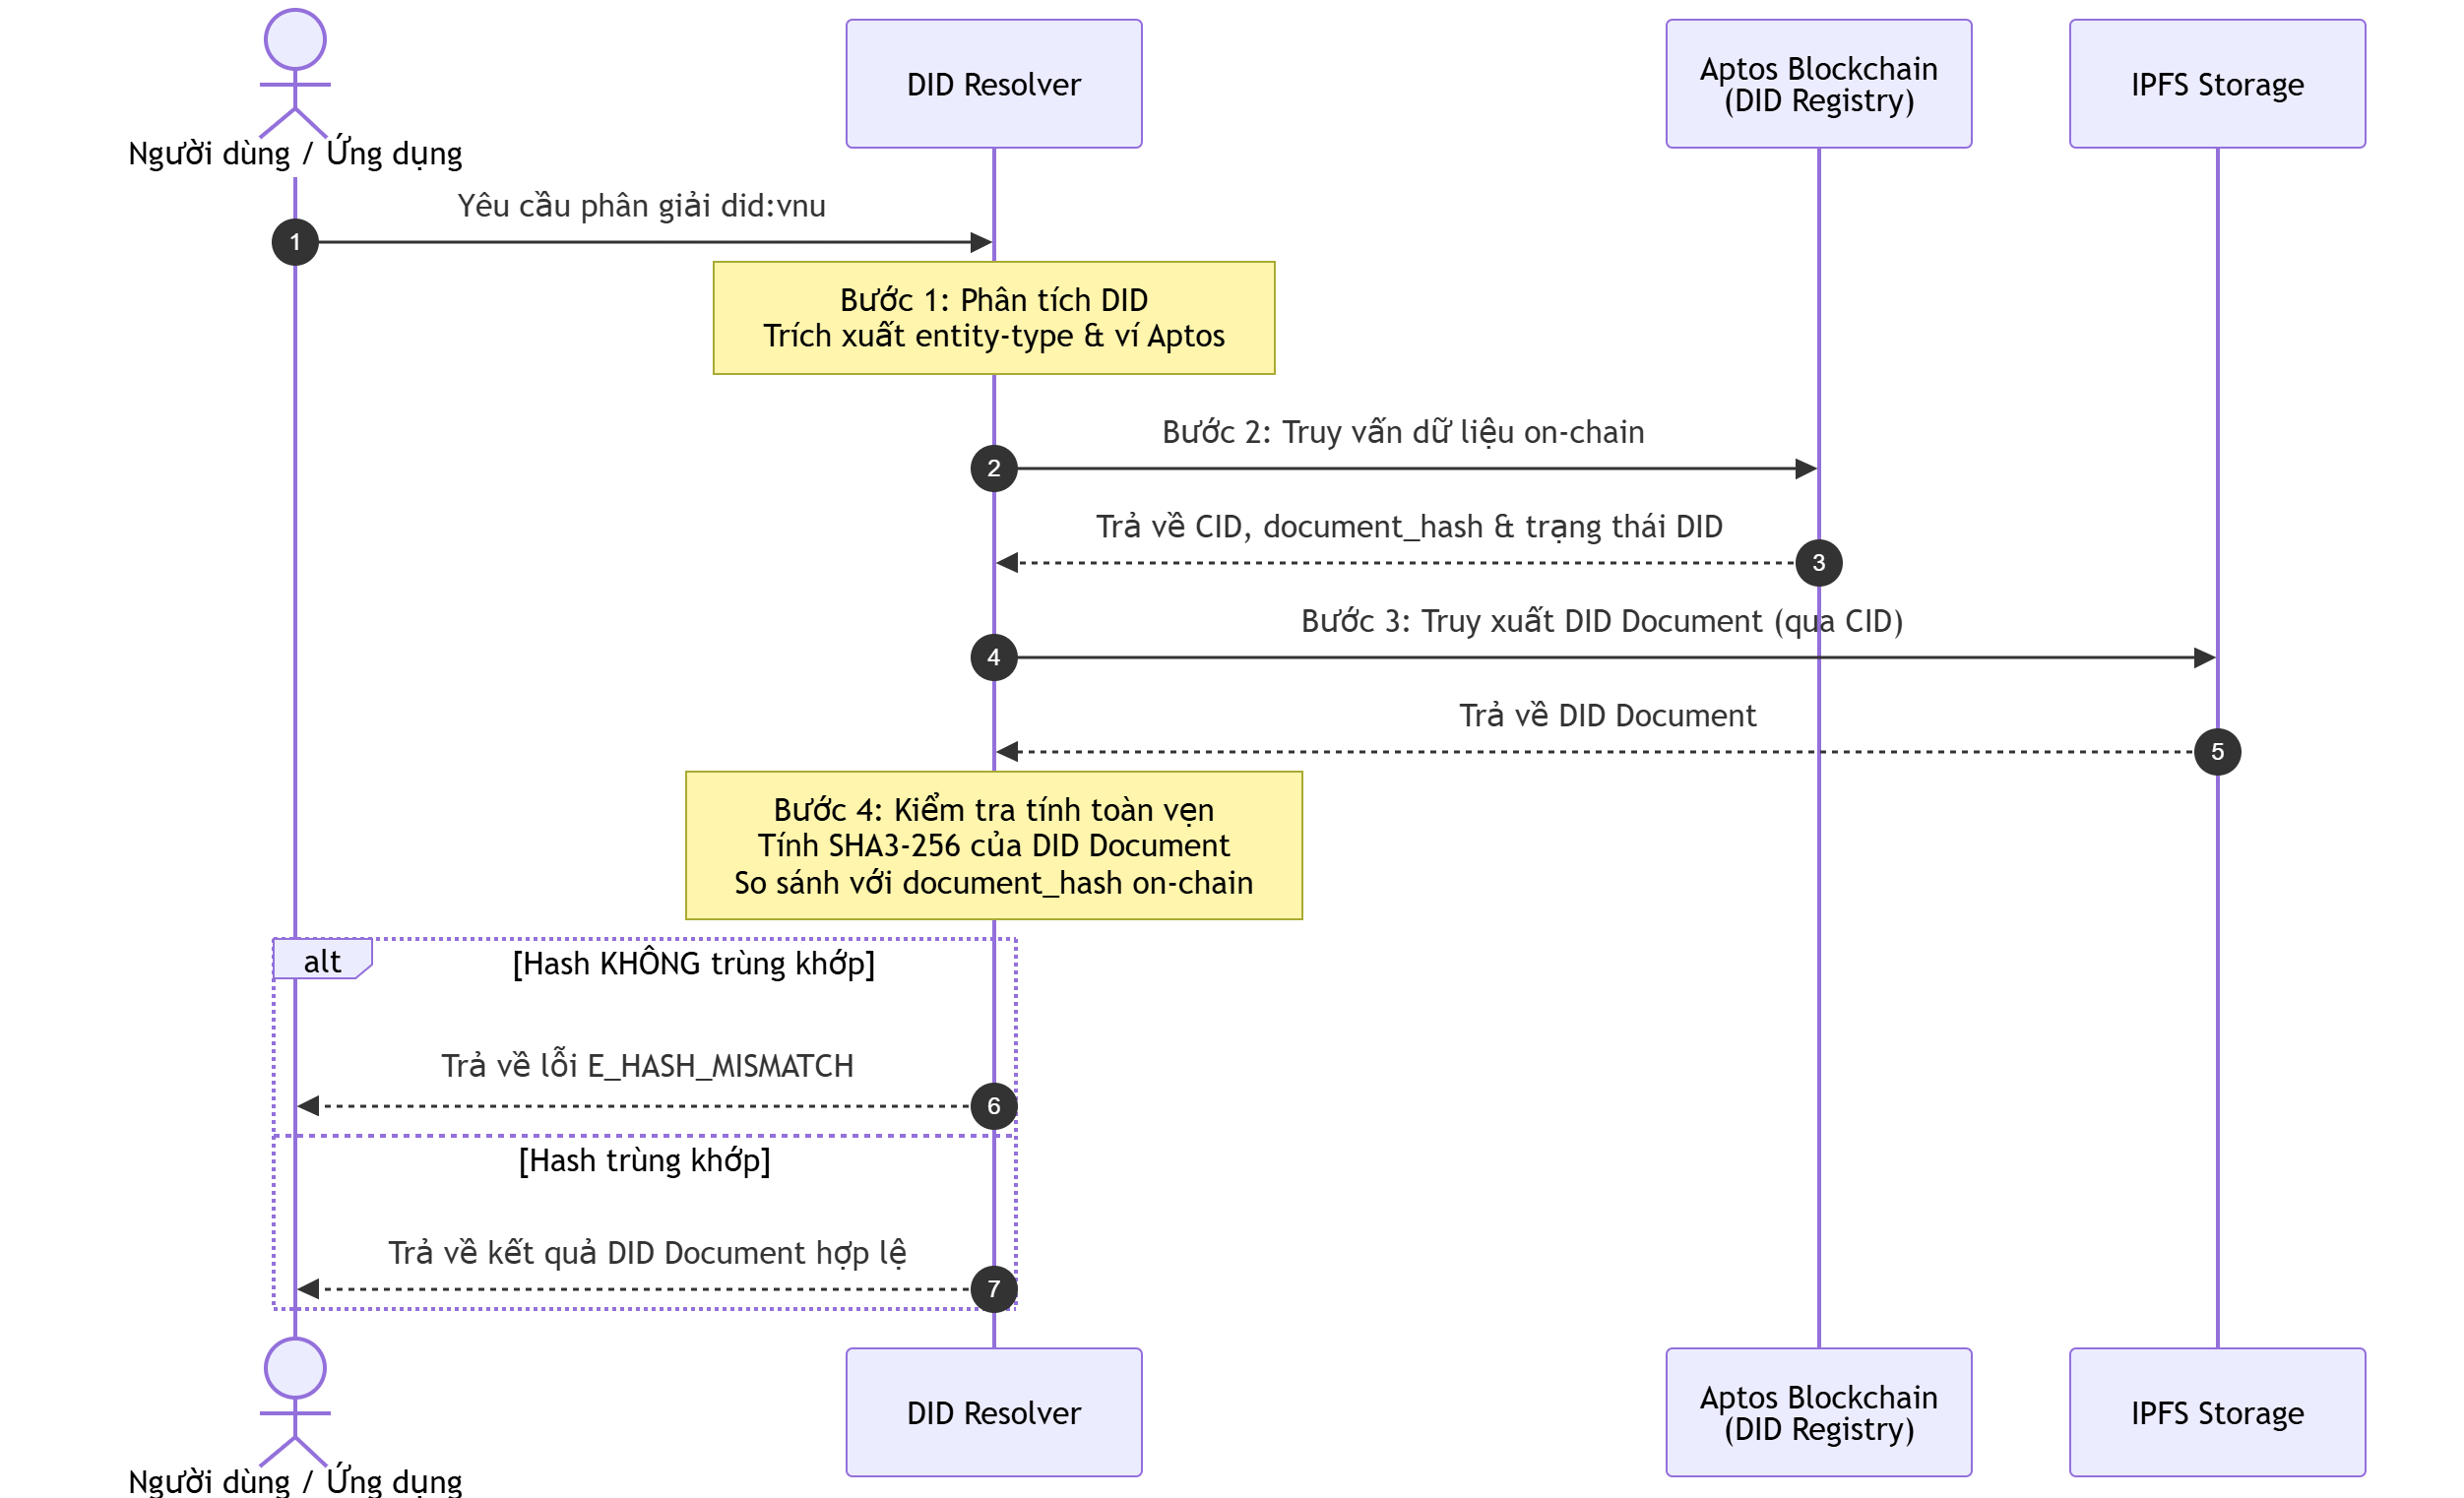
\includegraphics[width=0.9\textwidth]{images/did-resolution.png}
    \caption{Quy trình phân giải định danh trong phương thức \texttt{did:vnu}}
    \label{fig:did-resolution}
\end{figure}

Bước thứ tư là điểm phân biệt thiết kế này với các triển khai chỉ đọc tài liệu từ lớp lưu trữ mà không kiểm tra lại. Về lý thuyết, cơ chế định địa chỉ theo nội dung đã bảo đảm rằng nội dung không thể thay đổi mà giữ nguyên định danh. Trên thực tế, giữa bên xác minh và lớp lưu trữ còn có các cổng truy cập trung gian, và kết quả nhận về phụ thuộc vào cổng đó hoạt động đúng. Việc tính lại giá trị băm và đối chiếu với giá trị đã neo trên chuỗi loại bỏ sự phụ thuộc này: dù cổng nào trả về dữ liệu, bên xác minh vẫn phát hiện được sự không nhất quán.

\textbf{Về cơ chế xoay vòng khóa.} Khi một thực thể cần thay cặp khóa --- do nghi ngờ lộ khóa hoặc theo chu kỳ định kỳ --- thực thể đó dựng DID Document mới chứa khóa công khai mới, ghim lên lớp lưu trữ ngoài chuỗi để nhận định danh nội dung mới, rồi gọi thao tác cập nhật trên hợp đồng bằng chữ ký của khóa \emph{hiện tại}, qua đó chứng minh quyền kiểm soát định danh. Hợp đồng cập nhật định danh nội dung, giá trị băm và tăng số phiên bản. Các phiên bản trước vẫn được giữ, nhờ đó các chứng thực đã phát hành bằng khóa cũ vẫn xác minh được --- đáp ứng đúng yêu cầu đã nêu ở Mục 2.3.1 làm lý do thiết kế phương thức riêng. Thao tác cập nhật cũng nhận một tham số phiên bản kỳ vọng, nhằm phát hiện trường hợp hai cập nhật đồng thời ghi đè lên nhau.

\section{Quy trình xác minh}

\subsection{Bảy bước kiểm tra}

Quy trình xác minh được thiết kế theo nguyên tắc: mỗi bước kiểm tra một tính chất độc lập, và kết quả của từng bước được báo riêng. Cách này cho phép bên xác minh biết chính xác nguyên nhân thất bại --- điều mà Mục 2.8 xác định là một trong bốn khoảng trống của các hệ thống hiện có.

\begin{figure}[H]
    \centering
    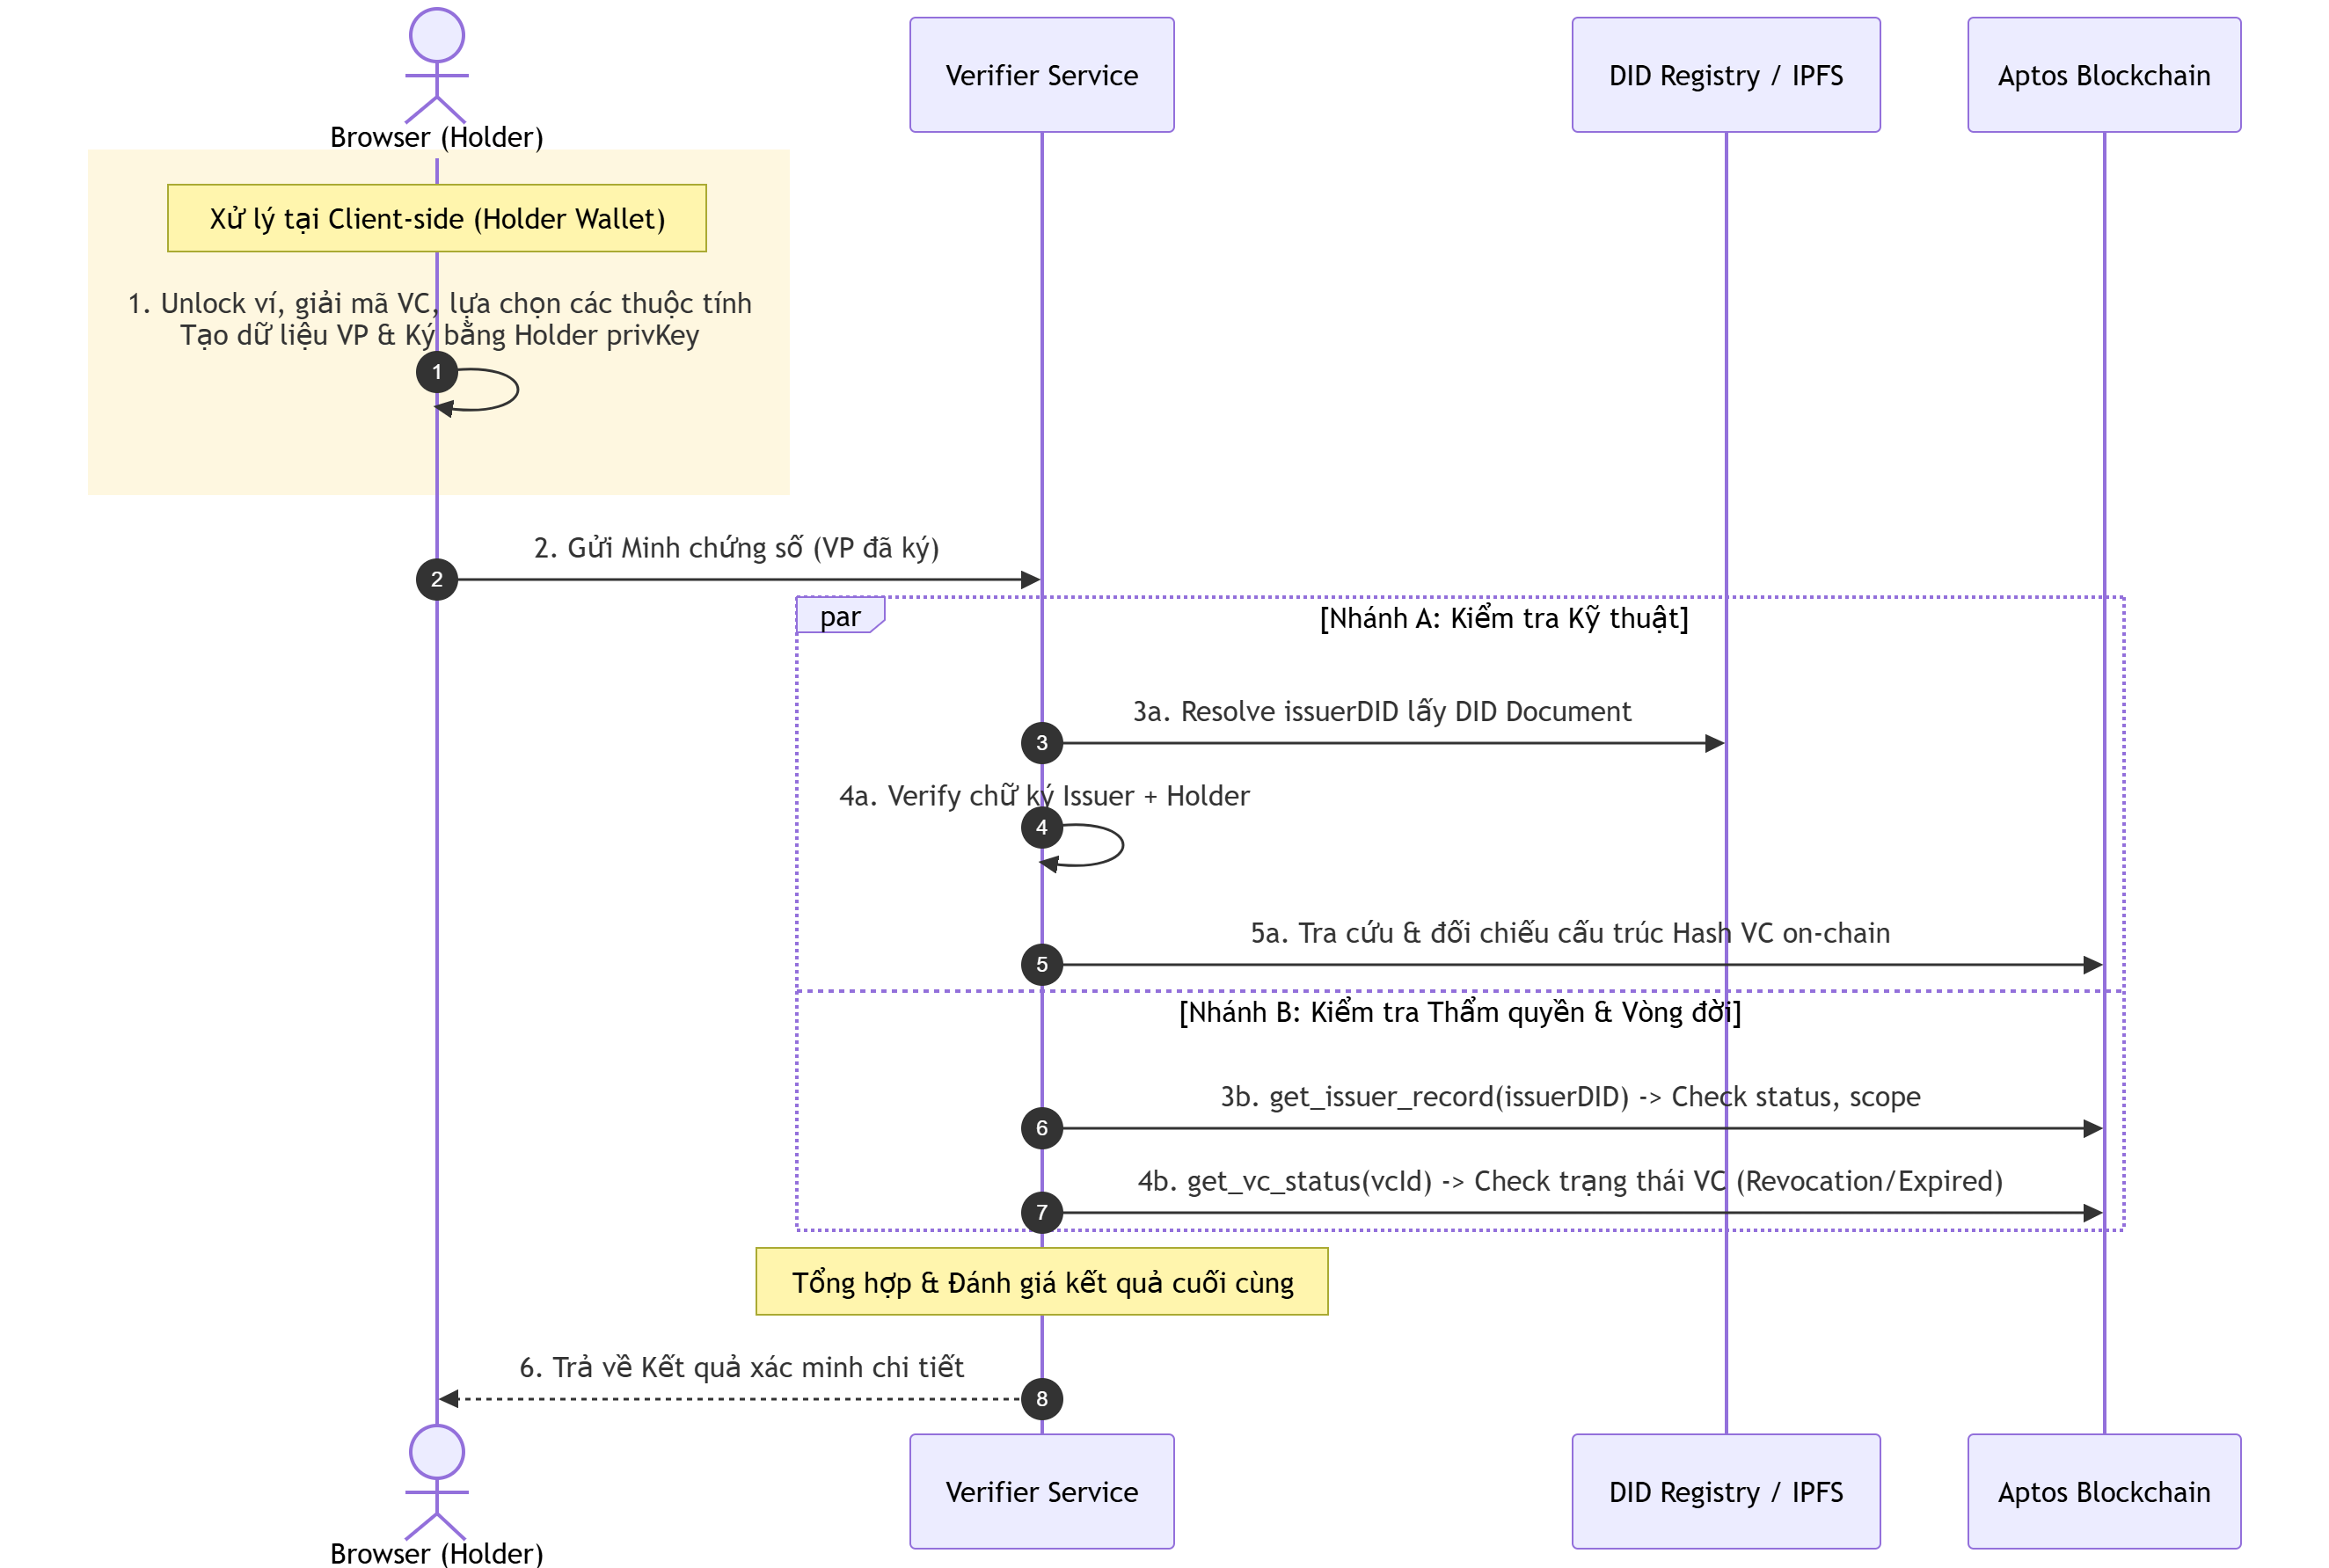
\includegraphics[width=1\textwidth]{images/seq_xac_minh_vp.png}
    \caption{Sơ đồ tuần tự quy trình trình bày và xác minh}
    \label{fig:seq_xac_minh_vp}
\end{figure}

Bảy bước, chia thành hai nhóm:

\noindent \textbf{Nhóm kỹ thuật --- tính toàn vẹn và quyền sở hữu:}

\begin{enumerate}
    \item \textbf{Truy xuất bản trình bày.} Tải nội dung bản trình bày từ lớp lưu trữ ngoài chuỗi theo định danh nội dung. Thất bại ở bước này nghĩa là dữ liệu không khả dụng, không phải dữ liệu không hợp lệ --- hai tình huống khác nhau cần được báo khác nhau.
    \item \textbf{Toàn vẹn bản trình bày.} Tính lại giá trị băm của nội dung nhận được và đối chiếu với giá trị đã ghi nhận.
    \item \textbf{Chữ ký của người trình bày.} Kiểm tra chữ ký trên bản trình bày bằng khóa công khai của chủ thể. Bước này xác lập rằng người trình bày đúng là chủ thể của chứng thực, không phải người đã lấy được một bản sao.
    \item \textbf{Trạng thái định danh của người trình bày.} Phân giải định danh của chủ thể và kiểm tra định danh đó còn hoạt động. Một định danh đã bị thu hồi --- chẳng hạn vì lộ khóa --- không được dùng để trình bày chứng thực.
\end{enumerate}

\noindent \textbf{Nhóm thẩm quyền và trạng thái:}

\begin{enumerate}
    \setcounter{enumi}{4}
    \item \textbf{Trạng thái hiệu lực của từng chứng thực.} Truy vấn trạng thái của từng chứng thực trong bản trình bày, bao gồm cả việc đánh giá thời điểm hết hạn.
    \item \textbf{Nội dung chứng thực khớp bản neo trên chuỗi.} Tính lại giá trị băm của nội dung chứng thực đang được trình bày và đối chiếu với giá trị băm đã neo trên chuỗi tại thời điểm cấp phát.
    \item \textbf{Thẩm quyền của bên phát hành.} Tra cứu trạng thái thẩm quyền của bên phát hành từng chứng thực trên chuỗi.
\end{enumerate}

Bước thứ sáu đáng được phân tích riêng, bởi nó là bước mà các hệ thống chỉ theo dõi trạng thái không có, và sự thiếu vắng của nó tạo ra một lỗ hổng cụ thể. Bước thứ năm trả lời câu hỏi {``}chứng thực này còn hiệu lực hay không{''}. Nó \emph{không} phát hiện được trường hợp nội dung chứng thực bị sửa sau khi cấp: nếu một bên nào đó sửa một trường trong nội dung --- chẳng hạn xếp loại hoặc điểm trung bình --- rồi ghim lại nội dung đã sửa, thì trạng thái của bản ghi trên chuỗi vẫn là {``}đang hiệu lực{''}, và cả bước thứ năm lẫn bước thứ bảy đều cho kết quả đạt. Phép kiểm duy nhất phát hiện được tình huống này là đối chiếu nội dung với giá trị băm đã neo.

Điều này không phải một khả năng lý thuyết. Mục 4.7 trình bày một kịch bản kiểm thử sửa nội dung trực tiếp trong chỉ mục rồi kiểm rằng bước toàn vẹn thất bại trong khi bước trạng thái vẫn đạt --- đúng để chứng minh rằng bước thứ sáu không dư thừa, và rằng một quy trình thiếu nó sẽ bỏ sót loại tấn công này.

\subsection{Ma trận kết quả xác minh}

Kết quả cuối cùng của quy trình là hợp lệ khi và chỉ khi cả bảy bước đều đạt. Tuy nhiên báo cáo xác minh không chỉ trả về một kết luận nhị phân mà trả về trạng thái của từng bước kèm chi tiết, bởi ba loại thất bại dưới đây có ý nghĩa xử lý hoàn toàn khác nhau.

\begin{longtable}{|p{2.3cm}|p{2.6cm}|p{2.2cm}|p{6.2cm}|}
\caption{Ma trận kết quả xác minh và ý nghĩa của từng loại thất bại}
\label{tab:verification-matrix} \\

\hline
\textbf{Nhóm kỹ thuật} & \textbf{Nhóm thẩm quyền} & \textbf{Kết quả} & \textbf{Ý nghĩa đối với bên xác minh} \\
\hline
\endfirsthead

\hline
\textbf{Nhóm kỹ thuật} & \textbf{Nhóm thẩm quyền} & \textbf{Kết quả} & \textbf{Ý nghĩa đối với bên xác minh} \\
\hline
\endhead

\hline
\endfoot

\hline
\endlastfoot

Đạt & Đạt & Hợp lệ
& Văn bằng hợp lệ cả về nội dung lẫn thẩm quyền cấp phát. Có thể chấp nhận.
\\ \hline

Không đạt & Đạt & Từ chối
& Nội dung bị sửa, chữ ký sai, hoặc bản trình bày do thực thể khác ký. Đây là dấu hiệu của gian lận chủ động và cần được báo cáo.
\\ \hline

Đạt & Không đạt & Từ chối
& Nội dung nguyên vẹn nhưng chứng thực đã bị thu hồi, đã hết hạn, hoặc bên phát hành không còn thẩm quyền. Báo cáo chỉ rõ nguyên nhân nào trong ba nguyên nhân này.
\\ \hline

Không đạt & Không đạt & Từ chối
& Báo cáo liệt kê đầy đủ các bước không đạt thay vì dừng ở bước đầu tiên, để bên xác minh thấy toàn bộ vấn đề.
\\ \hline

\end{longtable}


Sự phân biệt này có giá trị thực tiễn trực tiếp. Khi nội dung bị sửa, bên xác minh đang đối mặt với một hành vi gian lận chủ động và cần báo cáo. Khi chứng thực đã bị thu hồi, văn bằng đã từng hợp lệ nhưng không còn --- một tình huống hành chính bình thường. Khi bên phát hành mất thẩm quyền, bản thân chứng thực có thể vẫn đúng về nội dung, nhưng giá trị thể chế của nó cần được xem xét lại. Một kết quả {``}không hợp lệ{''} chung không cho phép phân biệt ba tình huống này.

\section{Mô hình đe dọa và các rào chắn}

Mục này kiểm tra lại tính đầy đủ của thiết kế bằng cách đi từ phía kẻ tấn công: liệt kê các hành vi mà một bên có ý đồ xấu có thể thực hiện, và xác định rào chắn nào ngăn mỗi hành vi đó.

\subsection{Giả định về năng lực của kẻ tấn công}

Mô hình đe dọa giả định kẻ tấn công có các năng lực sau: gửi được yêu cầu bất kỳ tới tầng dịch vụ, bao gồm yêu cầu có dữ liệu được dựng cố ý; đọc được mọi dữ liệu công khai trên chuỗi và trên lớp lưu trữ ngoài chuỗi khi biết định danh nội dung; và kiểm soát một tài khoản hợp lệ của chính mình, kèm khóa riêng tương ứng.

Mô hình \emph{không} giả định kẻ tấn công: chiếm được khóa riêng của người dùng khác; thực thi được mã trong trình duyệt của người dùng khác; hay làm sai lệch được trạng thái của chuỗi. Ba năng lực này nằm ngoài phạm vi phòng vệ của thiết kế, và hệ quả của chúng được thảo luận ở Mục 5.3.

Trong ba năng lực nằm ngoài phạm vi, một trường hợp cần được nêu riêng vì hệ quả của nó rộng hơn các trường hợp còn lại: \textbf{khóa riêng của một bên phát hành bị lộ}. Thiết kế hiện tại cho phép mỗi bên phát hành ký bằng một khóa duy nhất, nên kẻ chiếm được khóa đó cấp được chứng thực hợp lệ trong toàn bộ phạm vi thẩm quyền của đơn vị, cho tới khi thẩm quyền bị thu hồi. Đây là một đặc điểm chung của các hệ thống chứng nhận văn bằng dựa trên chữ ký đơn \cite{Saramago2021}, và nó không được giảm nhẹ bởi cơ chế hai bước ở Mục 3.4.4 --- cơ chế đó chỉ áp dụng cho việc chuyển quyền quản trị gốc.

Ba biện pháp giảm nhẹ \emph{một phần} có trong thiết kế: thẩm quyền có thời hạn nên thiệt hại bị chặn trên về thời gian; thẩm quyền có phạm vi nên thiệt hại bị chặn trên về loại văn bằng; và mọi chứng thực đã cấp đều thu hồi được, kể cả sau khi thẩm quyền của đơn vị đã bị thu hồi, theo nguyên tắc ở Mục 3.4.5. Biện pháp xử lý triệt để --- yêu cầu nhiều chữ ký hoặc chữ ký ngưỡng cho thao tác cấp phát --- nằm ngoài phạm vi bản thử nghiệm và được nêu tại Mục 5.4.

Một giới hạn về phương pháp cần được nêu ngay tại đây, trước khi trình bày kết quả. Mô hình đe dọa dưới đây do chính nghiên cứu định nghĩa, nên việc hệ thống chặn được toàn bộ các hành vi trong mô hình là \textbf{điều kiện cần chứ không phải điều kiện đủ} để kết luận về mức an toàn. Một mô hình tự định nghĩa luôn có nguy cơ bỏ sót đúng những hành vi mà người thiết kế không nghĩ tới --- và đó cũng là những hành vi nguy hiểm nhất. Để giảm nguy cơ này, các hành vi được liệt kê không xuất phát từ việc suy luận trên thiết kế mà từ ba nguồn độc lập hơn: các lỗi thật phát hiện trong đợt rà soát hợp đồng (Mục 4.3.5), các lỗi thật phát hiện khi đối chiếu hai cài đặt của tầng chỉ mục (Mục 4.4.1), và các loại tấn công được nêu trong tài liệu về định danh tự chủ \cite{Krul2024, Ambati2026}. Dù vậy, giới hạn vẫn còn và được thảo luận tại Mục 4.11.

\subsection{Các hành vi tấn công và rào chắn tương ứng}

\begin{longtable}{|c|p{3.6cm}|p{5.3cm}|p{3.4cm}|}
\caption{Mô hình đe dọa và rào chắn tương ứng}
\label{tab:threat-model} \\

\hline
\textbf{Mã} & \textbf{Hành vi tấn công} & \textbf{Rào chắn} & \textbf{Vị trí rào chắn} \\
\hline
\endfirsthead

\hline
\textbf{Mã} & \textbf{Hành vi tấn công} & \textbf{Rào chắn} & \textbf{Vị trí rào chắn} \\
\hline
\endhead

\hline
\endfoot

\hline
\endlastfoot

T1 & Tự khai là bên phát hành rồi cấp văn bằng
& Hợp đồng kiểm thẩm quyền trước khi ghi bản ghi; địa chỉ không có bản ghi thẩm quyền đang hoạt động thì thao tác thất bại
& Hợp đồng
\\ \hline

T2 & Cấp loại văn bằng ngoài phạm vi được phép
& Phép giao bit giữa loại văn bằng và mặt nạ phạm vi; kết quả bằng không thì từ chối
& Hợp đồng
\\ \hline

T3 & Tiếp tục cấp văn bằng sau khi thẩm quyền đã hết hạn
& Hợp đồng đối chiếu thời hạn ủy quyền với dấu thời gian của chuỗi
& Hợp đồng
\\ \hline

T4 & Khai báo mã giao dịch không tồn tại để tạo bản ghi về văn bằng không có trên chuỗi
& Bốn phép kiểm với nút đầy đủ trước khi ghi chỉ mục: giao dịch tồn tại; thành công; đúng hàm được gọi; đúng người gửi
& Tầng dịch vụ
\\ \hline

T5 & Tái sử dụng một giao dịch thật của chính mình nhưng thuộc loại thao tác khác
& Phép kiểm thứ ba trong T4: so khớp tên hàm trong phần tải của giao dịch với hàm mong đợi của tuyến
& Tầng dịch vụ
\\ \hline

T6 & Tái sử dụng giao dịch của người khác
& Phép kiểm thứ tư trong T4: so khớp người gửi giao dịch với tài khoản đang thực hiện yêu cầu
& Tầng dịch vụ
\\ \hline

T7 & Sửa nội dung văn bằng sau khi cấp rồi ghim lại nội dung đã sửa
& Bước thứ sáu của quy trình xác minh: tính lại giá trị băm của nội dung và đối chiếu với giá trị đã neo trên chuỗi
& Quy trình xác minh
\\ \hline

T8 & Trình bày một chứng thực của người khác đã lấy được bản sao
& Bước thứ ba của quy trình xác minh: chữ ký của người trình bày phải khớp khóa công khai của chủ thể ghi trong chứng thực
& Quy trình xác minh
\\ \hline

T9 & Khai báo giá trị băm sai để nội dung không khớp vẫn được chấp nhận
& Giá trị băm do máy khách khai báo đều được tính lại từ chính nội dung để đối chiếu trước khi ghi
& Tầng dịch vụ
\\ \hline

T10 & Mạo danh người khác khi đăng nhập bằng cách gửi lại chữ ký đã thu được
& Đăng nhập theo cơ chế thách thức -- đáp ứng với số dùng một lần có thời hạn; số đã dùng bị đánh dấu và không nhận lại
& Tầng dịch vụ
\\ \hline

T11 & Lợi dụng vai trò ghi trong phiên đăng nhập để thực hiện thao tác vượt quyền
& Các tuyến ghi có hệ quả trên chuỗi kiểm quyền trực tiếp trên chuỗi, không dựa vào vai trò trong phiên
& Tầng dịch vụ và hợp đồng
\\ \hline

T12 & Gán quyền gốc cho một địa chỉ không ai kiểm soát, qua đó làm mất năng lực quản trị
& Chuyển quyền gốc gồm hai bước; quyền chỉ chuyển sau khi người được đề cử tự ký để tiếp nhận
& Hợp đồng
\\ \hline

T13 & Đơn vị tự đình chỉ chứng thực rồi tự kích hoạt lại để xóa dấu vết
& Thao tác kích hoạt lại chỉ thuộc quản trị viên, không thuộc bên phát hành
& Hợp đồng
\\ \hline

T14 & Đăng ký một chuỗi định danh đã thuộc về thực thể khác
& Hợp đồng kiểm tính duy nhất của chuỗi định danh; đăng ký lại cho cùng một địa chỉ chỉ được phép sau khi định danh cũ đã bị thu hồi
& Hợp đồng
\\ \hline

T15 & Khai thác cổng truy cập trung gian để trả về nội dung khác nội dung đã đăng ký
& Phân giải định danh tính lại giá trị băm của tài liệu nhận được và đối chiếu với giá trị đã neo, bất kể nội dung đến từ cổng nào
& Quy trình phân giải
\\ \hline

\end{longtable}


Hai nhận xét về bảng trên.

Thứ nhất, \textbf{rào chắn cho các hành vi nghiêm trọng nhất đều nằm trong hợp đồng, không nằm trong tầng dịch vụ}. Điều này có chủ đích. Một rào chắn đặt ở tầng dịch vụ chỉ hiệu lực khi kẻ tấn công buộc phải đi qua dịch vụ đó; nhưng vì chuỗi là công khai, kẻ tấn công có thể gọi trực tiếp hợp đồng và bỏ qua hoàn toàn tầng dịch vụ. Vì vậy mọi quy tắc phân quyền phải được thi hành ở nơi không thể bị bỏ qua.

Thứ hai, \textbf{hành vi khai báo một tham chiếu giao dịch không tồn tại là hành vi đáng chú ý nhất về mặt thiết kế}. Trong một kiến trúc mà cơ sở dữ liệu chỉ là chỉ mục, mỗi bản ghi chỉ mục đều mang một tham chiếu tới giao dịch trên chuỗi đã tạo ra nó. Nếu tầng dịch vụ ghi nhận tham chiếu nào mà máy khách khai báo, thì máy khách chỉ cần gửi một chuỗi thập lục phân bất kỳ là tạo được một bản ghi về một văn bằng không tồn tại trên chuỗi. Rào chắn là bốn phép kiểm với nút đầy đủ trước khi ghi: giao dịch tồn tại; giao dịch thành công; hàm được gọi đúng là hàm mong đợi; và người gửi giao dịch khớp với tài khoản đang thực hiện yêu cầu. Thiếu phép kiểm thứ ba, kẻ tấn công có thể tái sử dụng một giao dịch thật của mình nhưng thuộc loại khác; thiếu phép kiểm thứ tư, họ có thể tái sử dụng giao dịch của người khác.

\section{Các đánh đổi trong quyết định thiết kế}

Mỗi quyết định kiến trúc đều kèm đánh đổi. Các đánh đổi dưới đây được ghi nhận tường minh --- không phải như hạn chế cần tránh nói tới, mà như kết quả của việc lựa chọn có chủ đích giữa những thuộc tính không thể đạt đồng thời.

\begin{longtable}{|p{2.9cm}|p{3.6cm}|p{3.6cm}|p{3.8cm}|}

\caption{Các đánh đổi trong quyết định thiết kế hệ thống
\label{tab:design-tradeoff}} \\

\hline
\textbf{Quyết định} &
\textbf{Thuộc tính thu được} &
\textbf{Thuộc tính phải hy sinh} &
\textbf{Cơ sở của lựa chọn} \\
\hline
\endfirsthead

\hline
\textbf{Quyết định} &
\textbf{Thuộc tính thu được} &
\textbf{Thuộc tính phải hy sinh} &
\textbf{Cơ sở của lựa chọn} \\
\hline
\endhead

\hline
\endfoot

\hline
\endlastfoot

Sổ đăng ký tin cậy trên chuỗi công khai thay cho cơ sở dữ liệu
&
Bên xác minh đọc được trạng thái thẩm quyền trực tiếp, không cần quan hệ trước với tổ chức nào; lịch sử quản trị không thể sửa
&
Chi phí giao dịch cho mỗi thao tác quản trị; trạng thái thẩm quyền trở thành thông tin công khai
&
Nếu sổ đăng ký là cơ sở dữ liệu thì bên xác minh lại phải tin tổ chức vận hành nó --- tức chỉ di chuyển sự phụ thuộc chứ không loại bỏ
\\ \hline

Một nguồn niềm tin gốc duy nhất
&
Mô hình quản trị đơn giản, trách nhiệm rõ ràng, phù hợp phạm vi kiểm chứng khái niệm
&
Tồn tại một điểm tập trung quyền lực quản trị
&
Phản ánh đúng cấu trúc thể chế hiện có của ĐHQGHN; kiến trúc phân lớp cho phép chuyển sang mô hình liên hợp mà không thay đổi ba lớp dưới
\\ \hline

Ví không lưu ký
&
Chủ thể là bên duy nhất ký được bản trình bày của mình, nhờ đó bước kiểm tra chữ ký của người trình bày có giá trị thật
&
Trải nghiệm phức tạp hơn; mất cụm từ khôi phục là mất quyền truy cập, không có cơ chế đặt lại
&
Mô hình lưu ký làm thay đổi tính chất an toàn mà hệ thống cung cấp, không chỉ làm giảm tính tự chủ về nguyên tắc
\\ \hline

Tách dữ liệu trên chuỗi và ngoài chuỗi
&
Chi phí lưu trữ thấp; không có dữ liệu cá nhân trên hạ tầng không thể xóa
&
Phụ thuộc vào tính khả dụng dài hạn của lớp lưu trữ ngoài chuỗi và cơ chế ghim
&
Ghi dữ liệu cá nhân lên hạ tầng bất biến khiến không thể thực hiện quyền của chủ thể dữ liệu theo quy định pháp luật
\\ \hline

Trạng thái theo từng bản ghi thay cho danh sách bit
&
Truy vấn trạng thái tức thời; thống nhất hạ tầng của ba sổ đăng ký trên cùng một lớp
&
Mỗi lần thu hồi là một giao dịch riêng; mỗi lần tra cứu để lại dấu vết về chứng thực được kiểm tra
&
Đơn giản hóa vận hành ở quy mô thử nghiệm; đây là điểm cần chuyển đổi khi mở rộng, và chỉ ảnh hưởng tới lớp chứng thực
\\ \hline

Chuẩn hóa JSON thay cho chuẩn hóa tập dữ liệu RDF
&
Triển khai được bằng mã ngắn, đồng nhất được giữa nhiều ngôn ngữ, dễ kiểm chứng tính tất định
&
Chỉ bảo đảm tương đương ở mức cú pháp; bên xác minh ngoài hệ thống cần mã kiểm tra riêng
&
Tương đương ngữ nghĩa của RDF yêu cầu bên xác minh triển khai toàn bộ phép xử lý JSON-LD, chi phí không tương xứng ở phạm vi hiện tại
\\ \hline

Giao diện dịch vụ theo kiểu REST thay cho giao thức truyền thông điệp giữa các tác nhân
&
Giảm đáng kể độ phức tạp triển khai và tích hợp
&
Khả năng tương tác giữa các hệ sinh thái thấp hơn kiến trúc tham chiếu đầy đủ
&
Phù hợp mục tiêu kiểm chứng mô hình quản trị; việc bổ sung giao thức truyền thông điệp không làm thay đổi kết luận về khung quản trị
\\ \hline

Giới hạn chuỗi ủy quyền ở hai cấp
&
Trách nhiệm luôn truy vết được tới một đơn vị cụ thể
&
Không biểu diễn được cấu trúc tổ chức sâu hơn hai cấp
&
Chuỗi ủy quyền sâu không giới hạn khiến việc truy vết trách nhiệm trở nên bất khả thi, trong khi lợi ích không rõ ràng
\\ \hline

\end{longtable}


Hai đánh đổi có ảnh hưởng lớn nhất cần được phân tích thêm.

\noindent \textbf{Ví không lưu ký.} Đây là đánh đổi tác động mạnh nhất tới trải nghiệm người dùng. Quyết định chọn mô hình không lưu ký xuất phát từ một quan sát ở Mục 2.3.4: trong mô hình lưu ký, bên vận hành có khả năng kỹ thuật để ký thay người dùng, nên toàn bộ lập luận về việc {``}chủ thể là bên duy nhất trình bày được chứng thực của mình{''} không còn thành lập. Nếu lập luận đó không thành lập, thì bước kiểm tra chữ ký của người trình bày trong quy trình xác minh mất ý nghĩa, và một trong ba thuộc tính tin cậy bị suy giảm. Nói cách khác, đây không phải một lựa chọn về nguyên tắc mà là một ràng buộc kỹ thuật: mô hình lưu ký làm thay đổi tính chất an toàn mà hệ thống cung cấp. Giá phải trả là người dùng gánh trách nhiệm bảo vệ khóa, và việc mất cụm từ khôi phục đồng nghĩa với mất quyền truy cập.

\noindent \textbf{Trạng thái theo từng bản ghi thay cho danh sách bit.} Như đã phân tích ở Mục 2.3.3, cơ chế danh sách bit của chuẩn W3C hiệu quả hơn về chi phí và cung cấp quyền riêng tư theo nhóm. Thiết kế này chọn cơ chế theo từng bản ghi vì nó cho phép truy vấn trạng thái tức thời và thống nhất hạ tầng quản lý định danh, thẩm quyền và trạng thái chứng thực trên cùng một lớp, giảm số thành phần cần vận hành. Hai cái giá phải trả là rõ ràng: mỗi lần thu hồi là một giao dịch riêng, nên chi phí tăng tuyến tính theo số lần thu hồi; và mỗi lần tra cứu để lại dấu vết về việc chứng thực nào đang được kiểm tra. Ở quy mô thử nghiệm, cả hai đều trong mức chấp nhận được; ở quy mô triển khai thật, đây là điểm cần chuyển đổi, và việc chuyển đổi khả thi vì nó chỉ ảnh hưởng tới lớp chứng thực.

\section{Đối chiếu với các kiến trúc tham chiếu}

\subsection{Những gì được kế thừa}

Kiến trúc đề xuất không được xây dựng từ đầu mà kế thừa có chọn lọc từ các mô hình đã phân tích ở Mục 2.7.

Từ Trust over IP \cite{ToIP_Stack2022}, nghiên cứu kế thừa tư duy phân lớp và --- quan trọng hơn --- quan điểm rằng quản trị phải được xem xét như một chiều kiến trúc độc lập ngay từ đầu, không phải một thành phần bổ sung sau cùng. Các thành phần phức tạp hơn của kiến trúc tham chiếu, cụ thể là giao thức truyền thông điệp giữa các tác nhân \cite{DIDComm2021} và kiến trúc dựa trên tác nhân, không được sử dụng nhằm giảm độ phức tạp triển khai trong phạm vi kiểm chứng khái niệm.

Từ mô hình niềm tin của EBSI \cite{EBSI_TrustModel}, nghiên cứu kế thừa hai nguyên tắc đã nêu ở Mục 2.7.2: hạ tầng ghi nhận các quyết định về niềm tin nhưng không tạo ra chúng, và mỗi bên xác minh tự quyết định họ chấp nhận gốc niềm tin nào. Nghiên cứu cũng kế thừa ý tưởng biểu diễn bản thân quan hệ ủy quyền thành một chứng thực có thể xác minh, thay vì chỉ một cờ trạng thái.

Điểm khác biệt cơ bản so với EBSI là nơi lưu trữ sổ đăng ký tin cậy. Thay vì một hạ tầng do một tổ chức vận hành, sổ đăng ký trong mô hình đề xuất là trạng thái của một hợp đồng trên chuỗi công khai, nên trạng thái thẩm quyền trở thành dữ liệu mà bất kỳ bên nào cũng đọc được trực tiếp. Điều này xử lý đúng khoảng trống thứ hai đã nêu ở Mục 2.8: giải quyết tầng niềm tin thể chế bằng cách tập trung hóa chỉ di chuyển vấn đề chứ không loại bỏ nó.

\subsection{So sánh ở mức thiết kế}

% Sáu cột ở cỡ chữ thường thì tràn lề phải ~20pt và chữ bị giãn rất xấu.
% Thu nhỏ cỡ chữ, giảm đệm cột và canh trái các ô thay vì bỏ bớt cột.
\begingroup
\footnotesize
\setlength{\tabcolsep}{3pt}
\begin{longtable}{|>{\raggedright\arraybackslash}p{2.8cm}|>{\raggedright\arraybackslash}p{2.4cm}|>{\raggedright\arraybackslash}p{2.5cm}|>{\raggedright\arraybackslash}p{2.3cm}|>{\raggedright\arraybackslash}p{2.3cm}|>{\raggedright\arraybackslash}p{2.3cm}|}
\caption{So sánh mô hình đề xuất với các hệ thống và kiến trúc tham chiếu}
\label{tab:system-comparison} \\

\hline
\textbf{Tiêu chí} & \textbf{Blockcerts} & \textbf{EDC / EBSI} & \textbf{Open Badges 3.0} & \textbf{Trust over IP} & \textbf{Mô hình đề xuất} \\
\hline
\endfirsthead

\hline
\textbf{Tiêu chí} & \textbf{Blockcerts} & \textbf{EDC / EBSI} & \textbf{Open Badges 3.0} & \textbf{Trust over IP} & \textbf{Mô hình đề xuất} \\
\hline
\endhead

\hline
\endfoot

\hline
\endlastfoot

Xác minh độc lập với bên phát hành
& Có
& Phụ thuộc hạ tầng khu vực
& Có
& Theo thiết kế
& Có
\\ \hline

Sổ đăng ký thẩm quyền
& Không có
& Có, do tổ chức vận hành
& Không có
& Mô tả khái niệm
& Có, là trạng thái hợp đồng trên chuỗi công khai
\\ \hline

Biểu diễn phạm vi cấp phát
& Không
& Theo lĩnh vực và địa bàn
& Không
& Mô tả khái niệm
& Mặt nạ bit theo loại văn bằng
\\ \hline

Thời hạn ủy quyền
& Không
& Theo chu kỳ kiểm định
& Không
& Mô tả khái niệm
& Trường thời hạn trong bản ghi, hợp đồng tự đối chiếu
\\ \hline

Ủy quyền nhiều cấp
& Không
& Có, qua tổ chức kiểm định
& Không
& Hoãn ở đặc tả truy vấn v2.0
& Có, với ba ràng buộc thi hành bởi hợp đồng
\\ \hline

Thu hồi thẩm quyền
& Không
& Có
& Không
& Mô tả khái niệm
& Có, trạng thái cập nhật trên chuỗi
\\ \hline

Cơ chế thu hồi chứng thực
& Danh sách do bên phát hành tự giữ
& Tập trung
& Tùy triển khai
& Không quy định
& Trạng thái theo từng bản ghi trên chuỗi
\\ \hline

Đối chiếu nội dung với bản neo khi xác minh
& Có
& Có
& Tùy triển khai
& Không quy định
& Có, là một bước riêng trong quy trình
\\ \hline

Phân biệt loại thất bại khi xác minh
& Không
& Không rõ
& Không
& Không quy định
& Có, báo cáo theo từng bước
\\ \hline

Chủ thể kiểm soát khóa
& Một phần
& Không
& Tùy triển khai
& Theo thiết kế
& Ví không lưu ký
\\ \hline

Tuân thủ chuẩn W3C DID / VC
& Một phần
& Một phần
& Có ở lớp chứng thực
& Tham chiếu chuẩn
& Tuân thủ, trừ phép chuẩn hóa và cơ chế trạng thái
\\ \hline

Cơ sở pháp lý đi kèm
& Không
& Có, theo khung eIDAS
& Không
& Không
& Chưa có; hành lang pháp lý trong nước đã hình thành
\\ \hline

\end{longtable}
\endgroup


Các mô hình hiện có chưa cân bằng được đồng thời ba thuộc tính: quản trị thẩm quyền, mức độ phi tập trung, và khả năng liên thông theo chuẩn mở. Blockcerts và Open Badges hỗ trợ xác minh độc lập nhưng thiếu quản trị bên phát hành; hạ tầng châu Âu có quản trị đầy đủ nhưng phụ thuộc hạ tầng tập trung; Trust over IP mô tả cả ba nhưng dừng ở mức kiến trúc tham chiếu.

\subsection{So sánh với mô hình truyền thống và mô hình định danh tự chủ thuần túy}

\begin{longtable}{|p{3.1cm}|p{3.5cm}|p{3.5cm}|p{3.5cm}|}
\caption{So sánh mô hình truyền thống, mô hình định danh tự chủ thuần túy và mô hình đề xuất}
\label{tab:traditional-ssi-comparison} \\

\hline
\textbf{Tiêu chí} & \textbf{Mô hình truyền thống} & \textbf{Định danh tự chủ thuần túy} & \textbf{Mô hình đề xuất} \\
\hline
\endfirsthead

\hline
\textbf{Tiêu chí} & \textbf{Mô hình truyền thống} & \textbf{Định danh tự chủ thuần túy} & \textbf{Mô hình đề xuất} \\
\hline
\endhead

\hline
\endfoot

\hline
\endlastfoot

Nơi đặt niềm tin
& Tổ chức trung gian
& Bằng chứng mật mã
& Bằng chứng mật mã cho nội dung; trạng thái công khai trên chuỗi cho thẩm quyền
\\ \hline

Điều kiện để xác minh
& Bên cấp phát hợp tác và còn tồn tại
& Truy cập được hạ tầng công bố khóa
& Truy cập được chuỗi và lớp lưu trữ ngoài chuỗi
\\ \hline

Chi phí một lần xác minh
& Tỉ lệ với số lần xác minh
& Gần như không đổi
& Gần như không đổi
\\ \hline

Phát hiện nội dung bị sửa
& Có, nếu đối chiếu được sổ gốc
& Có, bằng chữ ký
& Có, bằng chữ ký và bằng đối chiếu với giá trị băm đã neo
\\ \hline

Trả lời câu hỏi về thẩm quyền cấp phát
& Có, nhưng theo quy trình hành chính
& \textbf{Không}
& Có, bằng truy vấn công khai trên chuỗi
\\ \hline

Phạm vi và thời hạn của thẩm quyền
& Có trên văn bản, không kiểm chứng tự động được
& Không biểu diễn
& Biểu diễn tường minh và được hợp đồng thi hành
\\ \hline

Liên thông định danh giữa các cơ sở
& Không: mỗi cơ sở một mã riêng
& Có
& Có
\\ \hline

Chủ thể kiểm soát dữ liệu
& Không
& Có
& Có
\\ \hline

Dấu vết của thao tác quản trị
& Lưu nội bộ, có thể sửa
& Không có khái niệm quản trị
& Bất biến, công khai
\\ \hline

Phụ thuộc hạ tầng kỹ thuật
& Thấp
& Trung bình
& Cao: cần chuỗi, lớp lưu trữ ngoài chuỗi và ví
\\ \hline

Gánh nặng cho người học
& Thấp
& Cao: tự quản lý khóa
& Cao: tự quản lý khóa
\\ \hline

\end{longtable}


Bảng trên làm rõ vị trí của đóng góp. So với mô hình truyền thống, thay đổi nằm ở việc chuyển niềm tin từ trung gian sang bằng chứng, qua đó loại bỏ sự phụ thuộc vào bên cấp phát tại thời điểm xác minh. So với một hệ thống định danh tự chủ thuần túy, thay đổi nằm ở việc bổ sung lớp trả lời câu hỏi về thẩm quyền --- câu hỏi mà mật mã học không thể trả lời, và là lý do một hệ thống định danh tự chủ đúng về mặt kỹ thuật vẫn chưa đủ cho bài toán văn bằng.
